\section{Experiments} \label{sec:experiments} 

We have previously described the theory behind the methods we are implementing
to solve the authorship verification problem. In this section we will describe
in detail the experiments we performed to find the optimal hyperparameters and
network structure. We will test each method implemented against the external
validation set \gls{C}.

\subsection{Baseline Methods} \label{subsec:baseline_methods}

The implementation of both the \gls{SVM} and the Extended Delta method closely
resembles the implementation used by \citet{US}. There is however a big
difference with the application of the delta method. Contrary to the scenario
in \citep{US} where PAN data was used there is not an instance where we only
have 1 text per author. Therefore the original version of the delta method can
be used as described by \citet{evert2015towards}. This is the method where when
given a new text $t$ supposedly written by an author $\alpha \in \mathcal{A}$
his texts $T_\alpha$ are extracted and so is a set of texts not written by
him $\hat{T}_\alpha$ where $|\hat{T}_\alpha| = |T_\alpha|$. The text $t$ is
given to a \gls{KNN} classifier which determines if $t \in T_\alpha$ or $t \in
\hat{T}_\alpha$.

% TODO: Consider whether we should move some of the above description to method.


\subsubsection{Feature Selection}

The experiments performed on our baseline methods was centered around parameter
tuning. Not only parameters such as the $K$ in the extended delta method but
also the set of features supplied to the methods. Other methods such as random
forest has a built in filter for bad and noisy features. This is not the case
for both the \gls{SVM} and the extended delta method who does performs any kind
of quality analysis of the feature they are given. It is worst for the extended
delta method as that is just a distance metric that has no way of weighing
features. Therefore we chose to perform a feature selection for them rather than
just having them use the entire set available to them. Contrary to what was done
by \citet{US} this process did not consist of trying out some random selection
of features but rather a more systematic approach was used.

We started by generating a set of features. The feature set is simply a set of
n-grams. In order for us to find as good a feature set as possible we created a
large initial feature set to increase the feature search space. To generate the
features we used a corpus of text. Specifically we used the \gls{B} dataset as a
corpus. From the corpus we enumerated all the different n-grams in the different
categories and computed the frequency of each n-gram. The corpus had,

\begin{itemize}
    \item 27,535 different word-1-grams,
    \item 188,472 different word-2-grams,
    \item 2,178 different character-2-grams,
    \item 219 different \gls{POS}-tag-2-grams, and
    \item 524 special-character-2-grams.
\end{itemize}

The quantities here are large due to the size of the corpus and will continue
to rise as $n$ increases. Rather than extracting all of those features from
our texts we chose to focus on the n-grams with highest frequency as those are
probably the most important features. Specifically consider a case where a very
infrequent feature were chosen. That feature might only exist in the corpus and
in none of the texts in the test set. That feature would therefore be useless
in determining the authorship of those texts. Using the quantities listed above
as inspiration we generated a candidate feature set of 4950 features. The set
consisted of,

\begin{itemize}
    \item

        The frequencies of the 500 most frequent words,

    \item

        The frequencies of the 500 most frequent word-n-grams for $n \in \{2, 3,
        4\}$,

    \item

        The frequencies of the 300 most frequent character-n-grams for $n \in
        \{2, 3, ..., 10\}$,

    \item

        The frequencies of the 50 most frequent \gls{POS}-tag-n-grams for $n \in
        \{3, 4\}$, and

    \item

        The frequencies of the 50 most frequent special-character-n-grams for $n
        \in \{2, 3, 4\}$.

\end{itemize}

The quantities extracted reflects the inherent number of different n-grams of
that type. Since there are many more different words than characters there will
also be many more different word-n-grams than character-n-grams of the same
size. We therefore also use more of the most frequent word-n-grams. The sizes
of the different character n-grams we extracted was based on the amount used by
\citet{aalykke2016}. They found that character n-grams of size 8 worked very
well on MaComs data which is the reason why we chose to include char-n-grams
with n spanning the values from 1 to 10. \citet{US} showed that the when $n$
in word-n-grams reach a value of 4, the probability of that sequence actually
occurring in any given text is drastically reduced. A similar thing can be seen
with the special-character-n-grams where an increase in n would not contribute
anything. The reason for the small amount of \gls{POS}-tag-n-grams was that they
were a computationally expensive, as such a reduction in possible n-values had
to be made.

Having the features we could start doing our feature selection. The process
proved very computationally expensive. Having to check every combination of 4950
different features simply was not feasible. Therefore we implemented a greedy
algorithm instead in combination with using only a small dataset \gls{I} for the
feature selection.

The greedy algorithm as described by \citet{kanDeng} is a simple forward feature
selection. Having our previously created feature set we loop through each single
feature validating its accuracy when applied to each $\alpha \in \mathcal{A}$,
where $\mathcal{A}$ is the dataset \gls{I}. The validation on each author
$\alpha$ consists of fetching $T_{\alpha}$ and a set $\hat{T}_{\alpha} \subset
\overline{T}_\alpha$, where $|\hat{T}_\alpha| = |T_\alpha|$. Using these sets
of positive and negative cases we use k-fold cross validation to determine
the performance of the feature for that author $\alpha$. This is done for all
authors and when averaged we have the performance of that single feature. This
process is then repeated for all features. The best performing feature is then
added to a set of candidate features. In the next iteration we loop through all
the features again but we validate against each feature in combination with
the already selected features. This process is repeated until a set number of
features are selected. At that point the feature set that generated the highest
score is chosen.

Due to the increased run-time when using leave one out cross validation we had
to make use of some other model selection approach. Under normal circumstances
normal X-fold cross validation would work out fine but a complication arose when
doing this with the extended delta method. The reason for this was that there
was a scenario where an unlucky split of folds would cause a lot of error. A
generic example of this would be if we had a 2 class training set consisting
of 6 values evenly split between the 2 classes. In the case where we split
those 6 values into 3 folds there is a chance that a fold contains two values
of the same class which means that if $K = 3$ both of those wont ever be able
to classified correctly as there is only 1 of that class in the training set.
As such, stratified K fold cross validation is used instead as it uphold the
class distribution in its folds. While this is not a proglem for the \gls{SVM}
classifier we also opted the stratified K fold cross so we would more directly
compare the feature selection of the two models.

For both the \gls{SVM} and dxtended delta method, we ran this algorithm
until 450 features were selected. The \gls{SVM} performed its feature selection
using the default RBF kernel, a C with value of 1, and $\gamma =
\frac{1}{\text{n\_features}}$. Due to some authors having below 3 texts,
the default K value of \glspl{KNN} K parameter was set to 3 for the feature
selection.

The results of both the \gls{SVM} and the extended delta method feature selection can
be seen in Figure \ref{fig:fs_results}. The best number of selected feature were
220 for the SVM and 4 for the extended delta Method, scoring an accuracy of
0.697 and 0.672 respectively.

\begin{figure}
    \centering
    \textbf{Greedy Feature Selection}\par\medskip
    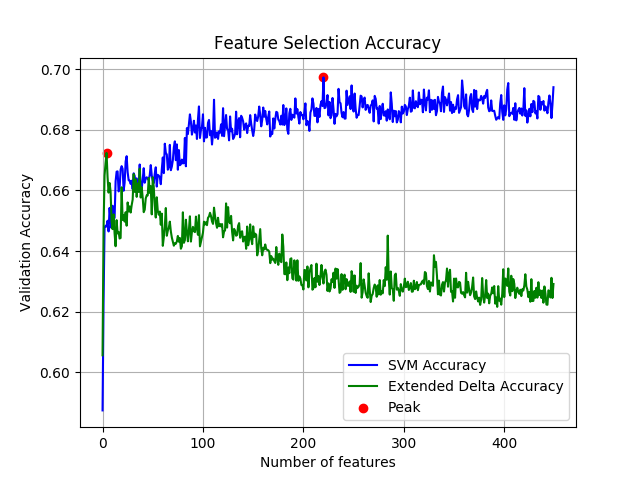
\includegraphics[scale=0.6]{./pictures/experiments/feature_selection}
    \caption{The process of the greedy feature selection of the SVM and the
        extended delta Method. The x axis shows the number of selected features
        so far in the search and the y axis the average accuracy when using that
        feature set for each author. The extended delta method peaks with a very
        small feature set while the \gls{SVM} needed more features to maximize
        accuracy.
    }
    \label{fig:fs_results}
\end{figure}


\subsubsection{Hyper Parameter Selection}\label{sec:hyp_select}

As mentioned in the previous section due to time constraints we were unable
to do the hyper parameter selection in parallel with the feature selection.
For that reason we chose to split it up selecting our features first and then
tuning the parameters based on those selected features. As before where we
searched for features in a set of features we now search for parameters in a set
of parameters. Recall that the \gls{SVM} need the $C$ and $\gamma$ parameters
and the extended delta method need the $p$ and $K$ parameters. We search for
parameters in a grid search of the values,

\begin{align}
    \text{SVM} &:
    \begin{array}{lr}
        C=\{10^{-3}, 10^{-1}, 10^{1}, 10^{3}, 10^{5}, 10^7\}\\
        \gamma=\{10^{-3}, 10^{-1}, 10^{1}, 10^{3}, 10^{5}, 10^7\}
    \end{array} \\
    \text{Extended Delta} &:
    \begin{array}{lr}
        p=\{1,2,3,4,5\}\\
        K=\{1,3,5,7,9,11,13,15\}
    \end{array}.
\end{align}

For each variation of the hyper parameters we average the performance of the
method over all unique authors in the training set in a manner very similar
to the feature selection. We make use of the same 3-fold stratified cross
validation and arrange each author with set of opposing set of texts. The
accuracy of each parameter configuration can be seen in Table \ref{table:KNN}
for the extended delta method, and Table \ref{table:SVM} for the \gls{SVM}. The
parameter search was performed on the \gls{J} dataset.

\begin{table}[h]
    \centering
    \textbf{\gls{KNN} Cross Validation Results}\par\medskip
    \begin{tabular}{|c|ccccc|}
        \hline
        \backslashbox{$K$}{$p$} & 1 & 2 & 3 & 4 & 5 \\\hline
        1 & \textbf{0.630} & 0.603 & 0.588 & 0.577 & 0.570\\
        3 & 0.628 & 0.589 & 0.572 & 0.565 & 0.555 \\
        5 & 0.621 & 0.576 & 0.559 & 0.549 & 0.545 \\
        7 & 0.612 & 0.564 & 0.546 & 0.537 & 0.533 \\
        9 & 0.600 & 0.554 & 0.537 & 0.527 & 0.524 \\
        11 & 0.587 & 0.542 & 0.527 & 0.520 & 0.517 \\
        13 & 0.581 & 0.537 & 0.524 & 0.517 & 0.514 \\
        15 & 0.571 & 0.532 & 0.519 & 0.514 & 0.512 \\\hline
    \end{tabular}
    \caption{The results from performing a grid search of the $p$ and $K$
        parameters of the \gls{KNN} algorithm.}
    \label{table:KNN}
\end{table}

\begin{table}[h]
    \centering
    \textbf{\gls{SVM} Cross Validation Results}\par\medskip
    \begin{tabular}{|c|cccccc|}
        \hline
        \backslashbox{$C$}{$\gamma$} & $10^{-3}$ & $10^{-1}$ & $10^{1}$ & $10^{3}$ & $10^{5}$ & $10^{7}$ \\\hline
         $10^{-3}$ & 0.626 & 0.626 & 0.626 & 0.641 & 0.558 & 0.500 \\
         $10^{-1}$ & 0.626 & 0.626 & 0.626 & 0.641 & 0.558 & 0.500 \\
         $10^{1}$  & 0.626 & 0.626 & 0.626 & \textbf{0.689} & 0.576 & 0.501 \\
         $10^{3}$  & 0.626 & 0.626 & 0.681 & 0.687 & 0.576 & 0.501 \\
         $10^{5}$  & 0.626 & 0.680 & 0.678 & 0.687 & 0.576 & 0.501 \\
         $10^{7}$  & 0.674 & 0.678 & 0.678 & 0.687 & 0.576 & 0.501 \\\hline
    \end{tabular}
    \caption{The results from performing a grid search for $C$ and $\gamma$ of
        the \gls{SVM} algorithm}
    \label{table:SVM}
\end{table}

We performed a validation of the methods on the \gls{C} dataset. While
applying these methods to a validation set wont change anything in terms of
the parameters we have selected. It will give us the ability to gauge the
accuracy of our methods when applied to a new never before seen test-set.
Using this untouched data set as the base the validation determines what text
from each author is the newest one ending up with a set of samples of the
form $(t, \alpha)$ where $t$ is a text and $\alpha$ is an author. For each
of these samples $T'_\alpha = T_\alpha \setminus \{t\}$ is extracted from
\gls{C}. Additionally another randomly sampled set $\hat{T}_\alpha \subset
\overline{T}_\alpha$ is extracted where $|\hat{T}_\alpha| = |T'_\alpha|$. Using
the combined set $T'_\alpha \cup \hat{T}_\alpha$, we can train the model in
question having provided it with both positive and negative examples of author
$\alpha$ writing style. To include samples that depict a student that used a
ghost writer we change the text we do our prediction on. For each sample there
is a probability that the sample will be regarded as negative. If that is the
case we pick out a random $t'$ where $t' \in (\overline{T}_\alpha \setminus
\hat{T}_\alpha)$ and predict on that where a correct prediction would be the
model say he did not write it. In the positive case we simply predict on $t$ and
a correct prediction would be the model saying he did write it. The results of
this process can be seen in Table \ref{tab:baseline-val-res}.

\begin{table}[h]
    \centering
    \begin{tabular}{|c|c|c|c|c|c|c||c|c|}
        \hline
        Split & Classifier & Params & TP & TN & FP & FN & \textbf{Accuracy} & \textbf{Accu Err} \\ \hline
        \multirow{2}{*}{50/50} & SVM & \{C:10, $\gamma$:1000\} &  759 & 692 & 308 & 241 & \textbf{0.7255} & \textbf{0.2583} \\ \cline{2-9} 
        & ED & \{K:1, p:1\} & 667 & 583 & 417 & 333 & \textbf{0.625} & \textbf{0.36353} \\ \hline
        \multirow{2}{*}{96/04} & SVM & \{C:10, $\gamma$:1000\} & 762 & 23 & 25 & 238 & \textbf{0.749} & \textbf{0.91187} \\ \cline{2-9} 
        & ED & \{K:1, p:1\} & 680 & 23 & 23 & 320 & \textbf{0.67208} & \textbf{0.93294} \\ \hline
    \end{tabular}
    \caption{The results of running our two baseline methods the \gls{SVM} and
        Extended Delta method, on the dataset \gls{C} the validation set.}
    \label{tab:baseline-val-res}
\end{table}

Unfortunately both of these methods are not suitable for the prediction system
described earlier and thus a to get it below the allowed accusation error was
not possible. While this is not ideal for comparative purposes it does lend
credence to the applicability of neural networks to this specific scenario.


\subsection{Deep Learning}

In the prediction system from Definition
\ref{def:weighted_average_prediction_system} we needed a function $f$ that
takes two texts and returns the probability that those texts are written
by the same author. As described earlier siamese \gls{NN}s are well
suited for comparing objects. In this Section we describe the experiments
we performed with different networks architectures and we will present
three different networks. The three networks are \gls{conv-char-NN} in
Section \ref{subsubsec:conv_char_nn}, \gls{conv-char-word-NN} in Section
\ref{subsubsec:conv_char_word_nn}, and \gls{rec-sent-NN} in Section
\ref{subsubsec:rec_sent_nn}.

The data we trained our networks on is described in Section \ref{sec:data}. We
trained the networks on the \gls{G} dataset that contains 3,000 authors. We used
early stopping based on a validation dataset \gls{H} that contains 500 authors.
Through experimentation we found that the validation dataset had to contain
completely different authors than the training dataset. In the beginning of
our project we had a validation set that contained different problem instances
(two texts to compare) from the training set but contained some of the same
authors. That lead to the validation set not being a very good estimate of the
networks performance on different authors than the ones seen during training.
The networks were therefore overfitting on the specific authors and we could not
see that in the validation datasets accuracy. All accuracy graphs shown in this
Section are based on a validation dataset with 500 completely unseen authors.

The general structure of our networks will be that they take two texts as input.
The texts are first embedded into a format that can be used by the network.
Then the texts are transformed into two sets of features representing the text
via a weight sharing network. Then the text representation will be combined
in some way and a dense network will take the combined representations and
decide whether or not the texts are written by the same author. We call the
different parts of the network \textit{Embedding}, \textit{Feature Extraction},
\textit{Combining} and \textit{Decision}.

When we show graphs of the networks we have produced we use specific names for
different layers in the networks. A glossary of the layer names and parameters
of the layers are shown in Table \ref{tab:glossary}.

\begin{landscape}
    \begin{table}
        \centering
        \textbf{Glossary}\par\medskip
        \begin{tabular}{|L{3cm}|L{9cm}|L{11cm}|}
            \hline
            \multicolumn{1}{|c|}{\textbf{Layer}}                               &
            \multicolumn{1}{|c|}{\textbf{Description}}                         &
            \multicolumn{1}{|c|}{\textbf{Actively Used Parameters}}           \\
            \hline

            Input                                                              &
            Serves as the entrypoint of the network, by receiving a set of
            texts and feeding it trough the network.                           &
            \begin{minipage}[t]{\linewidth}
            \begin{compactdesc}
                \item[Shape] The dimensions of each sample give to the input.
            \end{compactdesc}
            \end{minipage}                                                    \\
            \hline

            Embedding                                                          &
            Taking in an encoded sample, it produces a dense vector
            representation for each different. More details can be found in
            Section \ref{subsubsec:layers}.                                    &
            \begin{minipage}[t]{\linewidth}
            \begin{compactdesc}
                \item[Input Dim] Size of vocabulary.
                \item[Output Dim] Size of vector used to represent embedding.
            \end{compactdesc}
            \end{minipage}                                                    \\
            \hline

            Convolutional                                                      &
            Applies convolution to the data it recieves according to the
            decription, found in Section \ref{subsubsec:layers}.               &
            \begin{minipage}[t]{\linewidth}
            \begin{compactdesc}
                \item[Filters] Dimensionality of the output, ie. number of
                    filter from the convolution.
                \item[Kernel Size] Integer or list describing size of
                    convolution window.
                \item[Strides] Stride length of the convolutional window.
                \item[Activation] The activation function to be applied after
                    the convolution.
            \end{compactdesc}
            \end{minipage}                                                    \\
            \hline

            Global Max Pooling                                                 &
            Extracts the maximum value from each of the provided data          &
            No parameters.                                                    \\
            \hline

            Concatenation                                                      &
            As the name suggests, this layers simply concatenates the data it
            receives from different layers                                     &
            No parameters.                                                    \\
            \hline

            Merge                                                              &
            Merges its inputs, using a specified function to generate a single
            output.                                                            &
            \begin{minipage}[t]{\linewidth}
            \begin{compactdesc}
                \item[Function] The function used to merge the recieved data.
            \end{compactdesc}
            \end{minipage}                                                    \\
            \hline

            Dense                                                              &
            A simple fully connected layer, taking in data and applying the
            function described in Section \ref{sec:neurons}.                   &
            \begin{minipage}[t]{\linewidth}
            \begin{compactdesc}
                \item[Units] Number of neurons in in the layer.
                \item[Activation] The activation function to be applied.
            \end{compactdesc}
            \end{minipage}                                                    \\
            \hline

            Dropout                                                            &
            Drops a fraction it receives, with the goal of preventing
            overfitting.                                                       &
            \begin{minipage}[t]{\linewidth}
            \begin{compactdesc}
                \item[Rate] The fraction of data it receives dropped.
            \end{compactdesc}
            \end{minipage}                                                    \\
            \hline

            Lambda                                                             &
            Applies a specified function to the input it receives              &
            \begin{minipage}[t]{\linewidth}
            \begin{compactdesc}
                \item[Function] The function applied.
            \end{compactdesc}
            \end{minipage}                                                    \\
            \hline

            Reshape                                                            &
            Reshapes the data it receives.                                     &
            \begin{minipage}[t]{\linewidth}
            \begin{compactdesc}
                \item[Dim] Dimensionality to reshape to.
            \end{compactdesc}
            \end{minipage}                                                    \\
            \hline

            LSTM                                                               &
            A Long Short-Term Memory layer, which works according to the
            description in Section \ref{subsubsec:layers} is applied to the
            given data.                                                        &
            \begin{minipage}[t]{\linewidth}
            \begin{compactdesc}
                \item[Unit] Number of neurons in the layer.
            \end{compactdesc}
            \end{minipage}                                                    \\
            \hline
        \end{tabular}
        \caption{Glossary used when performing experiments, and creating their
            associated models \citep{chollet2015keras}.}
        \label{tab:glossary}
    \end{table}
\end{landscape}


\subsubsection{\glsdesc{conv-char-NN}}
\label{subsubsec:conv_char_nn}

The idea behind network \gls{conv-char-NN} is that we wanted to use convolutions
to look for n-grams in texts. Traditional authorship verification/attribution
is based on carefully engineered n-grams that are compared between two texts
\citep{stamatos2009}. Instead of choosing the n-grams ourselves we wanted the
network to learn which features are important for the authorship verification
task. The features are learned through convolutions. The convolutions look
at some number of characters at a time and gives a single output for those
characters. Assume for example that the network has learned that the character
sequence "ould " is important for deciding the author of a text. Then we
expect the network to react strongly to character sequences that looks
like "ould ". We have illustrated such a convolutional filter in Figure
\ref{fig:convolution_text_example}.

\begin{figure}
    \centering
    \textbf{Convolutions for Text Feature Extraction}\par\medskip
    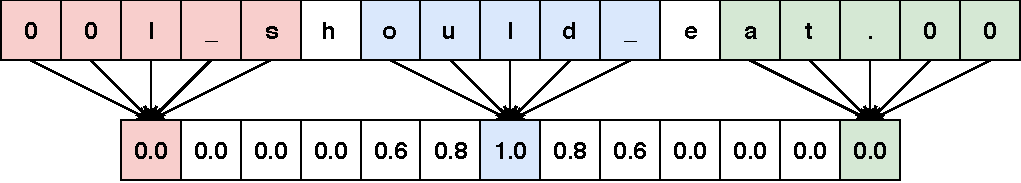
\includegraphics[width=\textwidth]{./pictures/experiments/convolution_example}
    \caption{Illustration of character level convolutions using a filter that
        looks for the character sequence "ould ". Notice that high values are
        produced when the characters the filter looks at match the characters it
        is looking for and low values are produced otherwise. We have
        illustrated 3 different filter locations but the filter is similarly
        placed in all possible locations. We have padded the text with zeros to
        get the same size output as input.}
    \label{fig:convolution_text_example}
\end{figure}

\begin{description}

    \item[Embedding:]

        The embedding takes as input a sequence of integers. Each different
        integer is a compact one-hot encoding of each character. The one-hot
        encoded character stream is embedded in a five dimensional space. The
        hope is that the layer will learn that similar characters should be
        placed close to each other in the output space and dissimilar characters
        should be placed far apart. The same embedding is performed on both of
        the input texts and the layer is therefore part of the siamese part of
        the network.

    \item[Feature Extraction:]

        Features are extracted from the two texts via a layer of convolutions
        with different sizes. We use both convolutions with a window size of
        8 and convolutions with a window size of 4. We use 700 of size 8 and
        500 of size 4. We used a window size of 8 since \citet{aalykke2016}
        found that n-grams of size 8 worked the best for Danish texts and we
        also added 4 so the network could look at smaller n-grams as well.
        We used a stride of 1 such that each convolutional filter could
        observe all parts of the texts and give an output for each one. The
        convolutional part of the network also shares weights such that the
        same features are extracted from both the input texts. We use the
        \gls{ReLu} activation function for the reasons described in Section
        \ref{subsubsec:activation_functions}.

        After the convolutional layer we added a global max pooling layer. The
        layer takes the maximum output of each convolutional filter. We do that
        as the output size of the convolutional layer depends on the length of
        the input text. The output of the max pooling layer is $700 + 500 =
        1200$ numbers, one for each convolutional filter. That means that the
        network learns to extract 1200 different features from each text.

    \item[Combining:]

        The features of the texts are combined using the absolute difference
        function. As described each text is represented as a vector of 1200
        features and to combine them we subtract them from each other and take
        the elementwise absolute difference.

    \item[Decision:]

        The decision part of the network consists of 4 dense layers each with
        500 neurons, a dropout layer and an output layer. The 4 dense layers
        also use the \gls{ReLu} activation function. The dropout layer is added
        just before the output layer and performs 30\% dropout to try to combat
        overfitting. The actual prediction is performed in the output layer.
        The output layer use the softmax function to return a probability
        distribution over the two possibilities that the texts are written by
        the same author and that they are written by different authors.

\end{description}

We have shown an illustration of the network in Figure \ref{fig:conv-char-NN}.
In the Figure we have illustrated the siamese part of the network as a blue box.
The 4 phases of the network is not illustrated in the Figure but it should be
possible to find them by reading the description above. We trained the network
on the dataset described in the Section \ref{sec:data} and in the beginning
of this Section. We used the \gls{Adam} optimizer during the training of the
network. We used a learning rate of $\eta = 0.0005$, half of what was suggested
by \citet{DBLP:journals/corr/KingmaB14}. We did that as we had problems with
neurons dying during the training of the network. Other than the learning rate
we used the parameters suggested in the article. That is, the remembering rates
were set to $\gamma_1 = 0.9$ and $\gamma_2 = 0.999$. As the error function we
used the binary cross-entropy function whose definition can be seen in Lemma
\eqref{eq:binary_ce}.

\begin{figure}
    \centering
    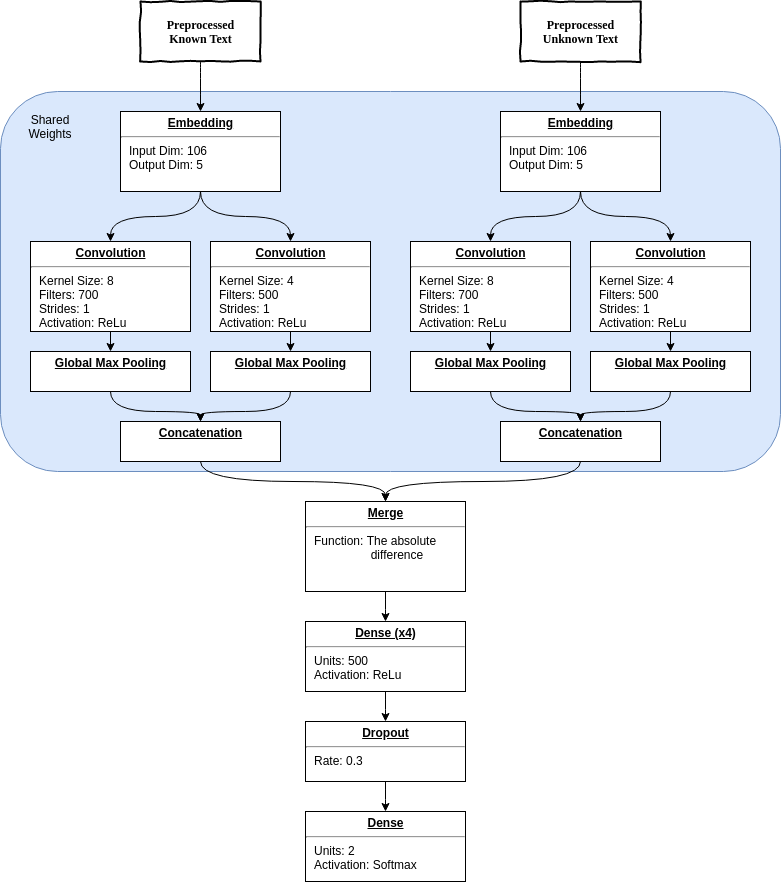
\includegraphics[width=\textwidth]{./pictures/experiments/conv_char_nn/model}
    \caption{The structure of network \gls{conv-char-NN}. Weights are
        shared by the embedding layers and the convolutional layers as shown by
        the blue box. The input to the network is at the top and the output is
        at the bottom. Information flows downwards through the layers. The final
        softmax layer produces a probability distribution over the two
        possibilities that the texts are either written by the same author or
        not.}
    \label{fig:conv-char-NN}
\end{figure}

\begin{lemma}[Binary Cross-Entropy]

    Let the loss function binary cross entropy be defined as,

    \begin{equation}\label{eq:binary_ce}
        L(y, p) = -(y \cdot \log(p) + (1- y)\cdot\log(1 - p)),
    \end{equation}

    where $y : \{0,1\}$ is a label and $p \in [0,1]$ is a predicted probability.

\end{lemma}

When we trained the network we were able to obtain a validation accuracy of
0.71773 in epoch 5. The training accuracy continued rising but we used early
stopping since the validation accuracy had stopped improving. We have shown
a graph of the training and validation accuracies during training in Figure
\ref{fig:conv-char-NN-accuracies}. During the training we used minibatch
learning with a minibatch size of 8. We used a size of 8 as that was the largest
batch size that could fit in the GPUs memory. During the training we padded
all texts with zeros such that all texts in each batch had the same length. We
did that as it is required by keras. We have shown the training and validation
accuracies during training in Figure \ref{fig:conv-char-NN-accuracies}.

\begin{figure}
    \centering
    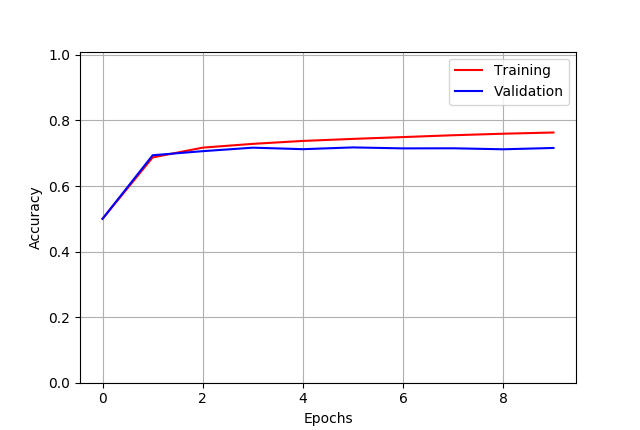
\includegraphics[width=0.6\textwidth]{./pictures/experiments/conv_char_nn/training_accuracy}
    \caption{The training and validation accuracy of \gls{conv-char-NN} during
        training. Each epoch contains several thousand minibatches which is why
        the training and validation accuracies rises so much in the first
        epoch.}
    \label{fig:conv-char-NN-accuracies}
\end{figure}

To arrive at the network architecture described above we experimented with
several similar architectures. We started with a network that was not too
far from the final one. All the work computed in this network was applied
to the same one-hot encoded character level as the final network was. The
feature extraction layer was however quite different. It made use of a single
convolutional layer consisting of 1000 filters with a window size of 10 the
selection of which did not have any proper argument and was selected solely
to determine the initial performance on the data. In addition to that the
combination part of the network also differed. Rather than computing the
absolute difference as was done in the final network, this initial network
simply concatenated the two siamese branches. If we let $t_f = \{t_1, t_2,
\dots, t_n\}$ be the extracted features of the text $t$, then the concatenation
would be computed by,

\begin{equation}
    combine(t, t') \mapsto (t_1, t_2, \dots, t_n, t'_1, t'_2, \dots t'_n)
\end{equation}

Finally the decision part of the network simply consisted of a single 500 neuron
dense network. The network gave promising results which is why we continued
working with it but it quickly overfitted on the training data so we added some
dropout. Like in the network presented above we added the dropout layer just
before the output layer and used 30\% dropout. That regularization allowed the
training accuracy and validation accuracy to follow each other for more epochs
making the final validation accuracy better.

We changed the combining function from a concatenation to a absolute difference
since the network would then not have to learn which features belonged to other
features. The new combination function is computed as,

\begin{equation}\label{eq:abs}
    combine(t, t') \mapsto \left(
        |t_0 - t'_0|, |t_1 - t'_1|, \dots, |t_n - t'_n|
    \right)^T.
\end{equation}

We also tried other combining functions such as the cosine difference but we
did not get any better results. After that change we changed the convolutional
filters from using 1000 filters of size 10 to using 500 filters of size 8 and
500 of size 4. We used those window sizes for the reasons described above. At
the same time we added more dense layers to the model. We again observed the
validation accuracy increasing further. Since our architecture seemed to work
well we scaled up the size of the network to having 4 dense layers instead of 1
as in the final network.

After expanding the network we wanted to figure out which features the network
were looking at. Since the convolutional layer (feature extractor) is followed
by a global max pool we knew that the feature a specific filter was looking
at could be determined by finding the maximum activation of that filter.
Unfortunately we found that the network were looking at metadata about the
texts. Specifically the network were looking at names and school class numbers.
Obviously a real ghost writer would make sure that the correct name and school
class were written on the assignment so in the real world those features should
not be used. The features are a product of the creation of the dataset we are
training on. Since different students assignments are combined to create the
negative samples we are training on (almost) all negative samples will have
different names written in them. Similarly (almost) all negative samples will
have different school classes written on them. Therefore such metadata will be
great features in our training dataset but not necessarily great features in
the real world. In Table \ref{tab:name_features} we have shown the activation
strings of the convolutional filter looking at Danish names.

\begin{table}
    \begin{tabular}{ll}
        \textbf{Activation String} & \textbf{Danish Surnames Matching} \\
        \hline
        \verb!adsen\n\n\n! & Madsen. \\
        \verb!ndsen\n\n\n! & Svendsen, Frandsen. \\
        \verb!elsen\n\n\n! & Nielsen, Mikkelsen. \\
        \verb!ersen\n\n\n! & Pedersen, Andersen, Petersen, Iversen, Jespersen. \\
        \verb!ansen\n\n\n! & Hansen, Christiansen, Johansen, Kristiansen. \\
        \verb!ensen\n\n\n! & Jensen, Christensen, S\o rensen, J\o rgensen, Kristensen,
                             Mortensen, Mogensen. \\
        \verb!arsen\n\n\n! & Larsen. \\
        \verb!ulsen\n\n\n! & Poulsen.
    \end{tabular}
    \caption{Showing the mapping from a convolutional filter looking at endings
        of common Danish surnames and the actual surnames. We found the list of
        the most common Danish surnames at \url{https://bit.ly/1d5WUmT}}
    \label{tab:name_features}
\end{table}

As described in Section \ref{sec:data} we tried to remove as much personal
information as possible from the texts by removing the first 200 characters and
by deleting names from the texts. When we trained the network again with those
preprocessing steps we got a substantial hit in network performance. However the
network were hopefully not looking at metadata anymore.


\subsubsection{\glsdesc{rec-sent-NN}}
\label{subsubsec:rec_sent_nn}

After having attempted a convolutional approach as was just described we
proceeded with some recurrent experiments as well. After having looked at
previous experiments described by \cite{qian:2018} which showed promise in
terms of authorship attribution we considered this a natural extension of
our convolutional approaches. Every \gls{RNN} experiment was performed on
the same data as the convolutional networks and the \textit{Embedding},
\textit{Feature Extraction}, \textit{Combining} and \textit{Comparing} structure
was used as well. The best model we generated can be seen depicted in Figure
\ref{fig:rec-sent-NN}. After 10 epochs this network peaked with a validation
accuracy of 0.657.

\begin{figure}
    \centering
    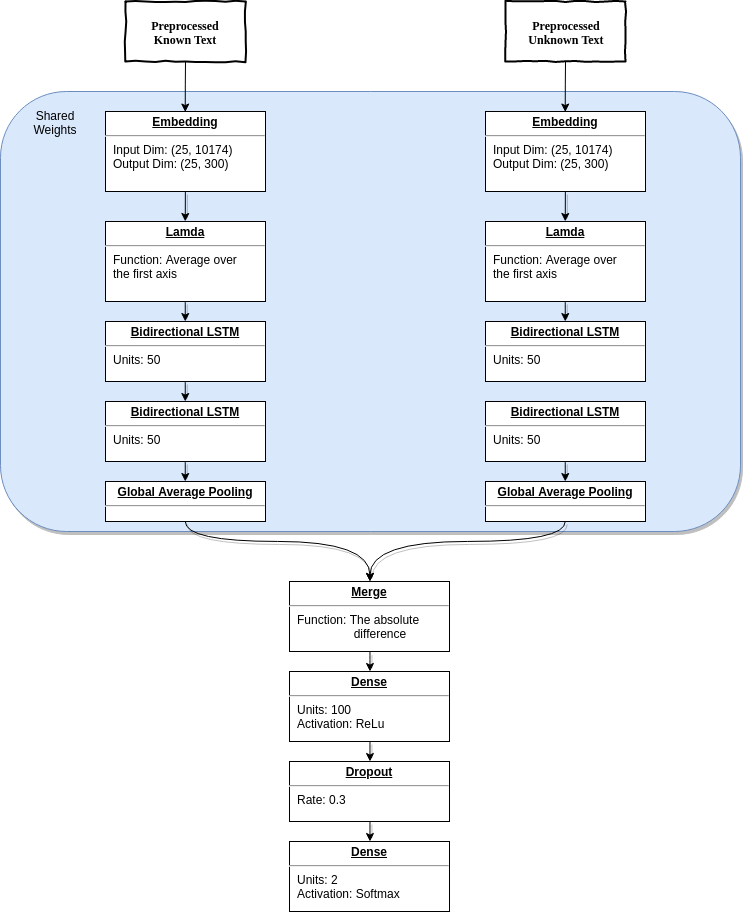
\includegraphics[width=\textwidth]{./pictures/experiments/rec_sent_nn/model}
    \caption{The structure of network \gls{rec-sent-NN}. The weights are shared
        from from the embedding layer all the way down to right before the two
        paths merge. The lambda layer takes each sentence and averages along
        the first axis causing the dimensionality to change from a matrix with
        25 rows and 300 columns to a column vector with 300 elements. The LSTM
        layers are bidirectional meaning its runs through the layer from both
        directions resulting in an output dimensionality twice the unit count
        of 50.
    \label{fig:rec-sent-NN}}
\end{figure}

\begin{description}

    \item[Embedding:]

        Like with the previous networks, this network is also a siamese neural
        network. It takes two texts as input and outputs the probability that
        they are written by the same author. As the title of this section
        suggests the network works on the sentence level rather than the
        character level. That clearly has consequences for the embedding part of
        the network.

        The input to the network is given as a sequence of sequences. The outer
        sequence consisting of sentences and the inner sequence consisting
        of the words in each sentence. In order for the dimensionality to
        work the amount of word in a sequence is padded or truncated such
        that they consist of 25 words each. An amount which was chosen based
        on the analysis of the training dataset \gls{B}. Contrary to earlier
        networks the embedded representations of these words were not trained
        as as part of the network. Pre-trained embedding produced by Facebook
        \footnote{\url{https://github.com/facebookresearch/fastText/blob
        /master/ pretrained-vectors.md}} using the method described by
        \citet{bojanowski2016enriching} was used instead. That resulted in each
        word being mapped to a 300 dimensional vector. At this point we have
        a sequence of sentences each containing a sequence of 300 dimensional
        word-embeddings. The network then proceeds to take the average of the
        word sequence contained within each sentence, resulting in each sentence
        being represented as the average of its words.

    \item[Feature Extraction:]

        The feature extraction part of this network consisted of recurrent
        layers. Specifically we used \gls{LSTM} layers described in
        Section \ref{layer:LSTM}. Two \glspl{LSTM} are placed right after
        one another. Both of them consists of 50 units and has the flag
        \textit{return\_sequences} set to true. This results in the output
        of all time-steps of the \gls{LSTM} being returned rather than just
        the last one giving us a sequence of outputs. We then proceed to
        combine all the returned sequences using a global average pooling
        layer. Rather than using a simple \gls{ReLu} which was the activation
        function we used on most layers for the reason explained in Section
        \ref{subsubsec:activation_functions} the \gls{LSTM} use 2 other
        activation functions. It use the tahn activation function from Equation
        \eqref{eq:tanh} after the last time step and the hard sigmoid activation
        function from Equation \eqref{eq:h_sig} after each individual time-step.
        This configuration is the default of the \gls{LSTM} layer provided by
        keras making the only change to the default parameters the number of
        units in the layer.

        The idea behind this feature extraction network was that we would
        extract 50 features from each sentence. We would then take the average
        over the whole text to extract 50 features that represented the author.
        Those features will then be used to combine the two texts. The feature
        extraction approach is very similar to what is done by
        \citet{qian:2018} who got very good results.

    \item[Combining:]

        Like the networks described in the earlier sections the combinations
        of our two siamese paths are done by taking the absolute difference
        of their two max-pooling outputs.

    \item[Decision:]

        The decision part of this network was kept quite simple. It simply
        consists of a single dense layer of 100 units which is then followed
        by a 30\% dropout layer for regularization. The result of the dropout
        layer is then provided to the last dense layer of 2 neurons using
        the soft-max activation function thus mapping it into a probability
        distribution. Since two neurons were used to depict the final output
        the loss function used for the network was binary cross-entropy paired
        with a \gls{Adam} optimizer with the learning rate of 0.0005, 50\% of
        the default value.

\end{description}

The path to this final design was a long one. The initial network designs
for our recurrent networks was based on a combination of the work done by
\citet{qian:2018} and our \gls{conv-char-NN} network described in Section
\ref{subsubsec:conv_char_nn}. We simply replaced the feature extraction
component in the network from convolutional layers to recurrent layers. In
addition that the first \gls{RNN} network also used the cosine similarity as its
method of combination on decision. It was when running this network, that the
main hindrance when using a character level recurrent network became apparent,
computation time. This first iteration of the network needed an estimated 140
hours to run through a single epoch. That was a very long time to train a
network and it was not feasible for us to try that in our limited time.

An attempt at saving training time was the inclusion of a convolutional layer
in the feature extraction part of the network. This would be placed before the
recurrent layers in an attempt to minimize the amount of data that was given to
the recurrent layers. The convolution used a window size of 8 and a stride of 8
meaning that each text would be 8 times smaller after the convolutional layer.
This did decrease the runtime but only resulted in an accuracy of 0.532 at its
peak. This was slightly increased when replacing the cosine similarity with a
series of dense layers instead and using a bidirectional \gls{LSTM} layer rather
than a single \gls{GRU} layer.

Instead of using convolutions to limit the text size we also tried changing
the linguistic level our network worked at. Again inspired by \cite{qian:2018}
we elevated our network from using the characters of the texts to using the
sentences. This sentence representation was achieved by doing as was described
in the \textbf{Embedding} part above. This approach significantly decreased
the runtime to around $1.5$ hours. But it also revealed the reason why a
recurrent network might not be the best choice for a task like this. The
validation error throughout training the network was not very high compared to
our earlier convolutional networks. The training accuracy also increased much
more than for the convolutional networks while the validation accuracy quickly
stalled. It therefore seemed like this approach was very prone to overfitting on
particular authors. This lead to the final network described above. This network
included an extra bidirectional \gls{LSTM} layer, and the 0.3 dropout for extra
generalization.

As mentioned this final network yielded the accuracy initially described,
0.657 after 10 epochs. 


\subsubsection{\glsdesc{conv-char-word-NN}}
\label{subsubsec:conv_char_word_nn}

The last network we produced, is what we call \gls{conv-char-word-NN}.
This network is very reminiscent of \gls{conv-char-NN}, mostly due to
its convolutional nature. This network was an attempt at expanding
on the successful architecture of \gls{conv-char-NN}. Applied to the 
same data as the previous networks, we got a maximum accuracy of 0.697
on the second epoch. The design of the network in the different parts was
as follows

\begin{description}

    \item[Embedding:]

    Like in \gls{conv-char-NN} the embedding layers takes in a text as a
    stream of characters, where they are then mapped to a 5 dimensional vector
    space. There is not a very big difference here. In addition to that however,
    we also added the word channel used in \gls{rec-sent-NN}. This works in
    exactly the same way. It uses the pre-trained embeddings mentioned to map
    each word of the text in addition to mapping the characters. This is the
    basic idea of this network, a multi-channeled convolutional approach. Thus
    the network doesn't only take 2 inputs, in the form of two texts. It takes 4
    inputs, a character input for each each and a word input for each text. Both
    of these channels have their own path through the network. Which for ease of
    understanding can be seen as two different siamese networks.

    \item[Feature Extraction:]

    The feature extraction done in this network differs between the character
    network and the word network. Like previously, we make use of two different
    convolutional layers in the character network. They have a sliding windows
    size of 8 and 4, and a filter size of 200. This combination of window sizes
    had proven to work quite in the \gls{conv-char-NN}. It was because of this
    we saw no reason to actually change it, as the creation of this network was
    done in an additive manner. The addition can of course be found in the word
    network. The embedded stream of words are given to its own convolutional
    layer with a sliding window size of 8, and a filter size of 100.

    \item[Combining:]

    Due to the addition of the extra word network, the combining of step is
    has an additional step. The network initially combine the output of both
    the word and the character sub-networks. This is done by concatenating
    the output of the two convolutional layers in the character network, and
    the single convolutional layer in the word network. This results in two
    concatenated sets, one for each of the two texts. The elementwise absolute
    difference of the two sets are then computed, and passed along to the
    decision part of the network.

    \item[Decision:]

    The decision part of this network is simply 2, 500 unit fully connected
    layers followed by a 0.3 dropout layer. The output of that dropout layer
    is then given the 2 unit soft-max layer, for the final decision.

\end{description}

The path gone through to reach this design was a rather short one, compared
to to the two described above. The design of this network was derived based
on a combination of the other two network, the \gls{conv-char-NN}, and
\gls{rec-sent-NN}. The convolutional approach used on \gls{conv-char-NN},
showed promise, and this network was an attempt to improve on that.

Initially these alternations were small. They took the form on a different
amount of convolutional layers, with a differing amount of sliding window sizes.
These small changes also included the addition of regularization measures,
such as dropout layers. The largest change came when we incorporated the
multi-channel approach used in \gls{rec-sent-NN}. The thought process was,
that if character were good features for this task, another channel would
only provide additively better results. This was what yielded the network
described above, which works on the character level and the word level. 3
channel convolutional network were also produced during experimentation. Results
from that seemed to indicate that the linguistic level of sentences were too
high, thus hurting the model.

\subsection{Prediction System}

Our prediction system has several hyperparameters we have to choose to get
the best results. We recall that MaCom wanted a system that had an accusation
error of less than 10\%. We can use the threshold parameter $\theta$ in the
prediction system to control how many people we accuse. The best parameters
for the prediction system is those parameters that gives the highest accuracy
subject to the constraint that the accusation error should be less than 10\%. To
tune the parameters we use the dataset \gls{H}. From that dataset we constructed
a set of tuples $(\alpha, t_u)$ where $\alpha$ is a candidate author and $t_u$
is a text of unknown authorship. We let the set of tuples be known as $V$. None
of the authors in \gls{H} has been seen by the networks during training and none
of the texts $t_u$ has been seen by the networks during training. The parameters
that maximize the accuracy subject to the bounded accusation error is the same
as the parameters that minimize the error rate subject to the bounded accusation
error. That optimization problem is,

\begin{equation}
    \label{eq:prediction_system_minimization}
    \begin{aligned}
        & \underset{\theta, x}{\text{minimize}}
        & & \sum_{(\alpha, t_u) \in V} \left|
            P_x(T_\alpha \setminus \{t_u\}, t_u, \theta) -
            \mathbbm{1}_{T_\alpha}(t_u)
        \right| \\
        & \text{subject to}
        & & \frac{\sum_{(\alpha, t_u) \in V} \mathbbm{1}_{T_\alpha}(t_u) \cdot
            \left(1 - P_x(T_\alpha \setminus \{t_u\}, t_u, \theta)\right)}
{\sum_{(\alpha, t_u) \in V} (1 - P_x(T_\alpha \setminus \{t_u\}, t_u, \theta)} <
            \frac{1}{10}
    \end{aligned}
\end{equation}

In the optimization problem we fix the network $f$ we validate like we did
when defining the prediction systems. The expression we minimize is the
number of errors made in prediction over the validation set $V$. Consider a
problem $(\alpha, t_u) \in V$ where $t_u \in T_\alpha$. Then we know that
$\mathbbm{1}_{T_\alpha}(t_u) = 1$ from the definition of the indicator function
then if the prediction system returns the correct result 1 we have,

\begin{equation}
    e = \left|
        P_x(T_\alpha \setminus \{t_u\}, t_u, \theta) -
        \mathbbm{1}_{T_\alpha}(t_u)
    \right| = |1 - 1| = 0,
\end{equation}

and if the prediction system returns the incorrect result 0 we have,

\begin{equation}
    e = \left|
        P_x(T_\alpha \setminus \{t_u\}, t_u, \theta) -
        \mathbbm{1}_{T_\alpha}(t_u)
    \right| = |0 - 1| = 1.
\end{equation}

Similarly for a problem $(\alpha, t_u) \in V$ where $t_u \notin T_\alpha$ we
know that $\mathbbm{1}_{T_\alpha}(t_u) = 0$ from the definition of the indicator
function. Then if the prediction system returns the correct result 0 we have,

\begin{equation}
    e = \left|
        P_x(T_\alpha \setminus \{t_u\}, t_u, \theta) -
        \mathbbm{1}_{T_\alpha}(t_u)
    \right| = |0 - 0| = 0, \end{equation}

and if the prediction system returns the incorrect result 1 we have,

\begin{equation}
    e = \left|
        P_x(T_\alpha \setminus \{t_u\}, t_u, \theta) -
        \mathbbm{1}_{T_\alpha}(t_u)
    \right| = |1 - 0| = 1.
\end{equation}

That is the expression we minimize is 0 whenever there is no error and 1
whenever there is an error. So we minimize the number of errors we make. The
subject to expression makes sure that the fraction of false accusations we make
is less than $10\%$ of the accusations we make. The expression should be read
as,

\begin{equation}
    \frac{\textit{false accusations}}{\textit{total accusations}} < \frac{1}{10}
\end{equation}

Consider the numerator of the fraction on the left hand side,

\begin{equation}
    \textit{false accusations} = \sum_{(\alpha, t_u) \in V}
    \mathbbm{1}_{T_\alpha}(t_u) \cdot
    \left(1 - P_x(T_\alpha \setminus \{t_u\}, t_u, \theta)\right).
\end{equation}

For a $(\alpha, t_u) \in V$ where $t_u \in T_\alpha$ we have that
$\mathbbm{1}_{T_\alpha}(t_u) = 1$ then if $P$ is correct it returns 1 and we
get,

\begin{equation}
    \mathbbm{1}_{T_\alpha}(t_u) \cdot
    \left(1 - P_x(T_\alpha \setminus \{t_u\}, t_u, \theta)\right) =
    1 \cdot (1 - 1) = 0,
\end{equation}

and if $P$ is incorrect and returns 0 we have,

\begin{equation}
    \mathbbm{1}_{T_\alpha}(t_u) \cdot
    \left(1 - P_x(T_\alpha \setminus \{t_u\}, t_u, \theta)\right) =
    1 \cdot (1 - 0) = 1.
\end{equation}

Similarly for a $(\alpha, t_u) \in V$ where $t_u \in T_\alpha$ we have that
$\mathbbm{1}_{T_\alpha}(t_u) = 0$ and therefore the expression is always
0. Therefore the expression is 1 whenever we have a false accusation and 0
otherwise. The right hand side of the inequality simply counts the number of
accusations by inverting the output of $P$ and divides that by 10. So the
condition makes sure that only 10\% of the accusations we make are false
accusations.

We have run our prediction system on several of the networks we trained as
part of our experiments. For each of the networks we present several graphs
showing their performance for different prediction systems and thresholds and
we report the best configuration for that network. The dataset we use to tune
$\theta$ and the weight function $w$ are \gls{F}. The set consists of 2,000
previously unseen authors. For each author we generate two problems meaning that
we end up with 4,000 different problems. For each of the authors we generate a
positive sample by taking the newest text as the unknown text and a negative
sample by choosing a random text from some other author in the set. That is
we have a 0.5 split between positive and negative samples. We also tried our
prediction system on another validation set. In the real world it has been
estimated that 4\% of turn ins for the \gls{SRP} are written by "ghost writers"
\footnote{https://politiken.dk/indland/uddannelse/art5603163/Gymnasieelever-\%C2
\% BBSnyderi-beviser-hvor-vanvittig-betydningsfuld-SRP-er-blevet\%C2\%AB}. We
therefore also wanted to find the $\theta$ and $w$ for a validation set with
only 4\% negative samples instead of 50\% negative samples. We generated 2,000
positive samples as before and then for each sample we added a negative sample
with a 4\% chance.


\subsubsection{\glsdesc{conv-char-NN}}
\label{subsubsec:prediction_system_conv-char-NN}

The first network we tuned hyperparameters for were the network presented
in Figure \ref{fig:conv-char-NN}. The network used only convolutions on the
character level to extract features and used a dense network to decide whether
or not the texts were written by the same author. We have shown the accuracy
and accusation error for the dataset containing 50\% negatives in Figure
\ref{fig:conv-char-NN-pred-50} and for the dataset containing 4\% negatives in
Figure \ref{fig:conv-char-NN-pred-4}.

\begin{figure}
    \centering
    \textbf{Prediction System Results for 0.5 Split, \glsdesc{conv-char-NN}}\par\medskip
    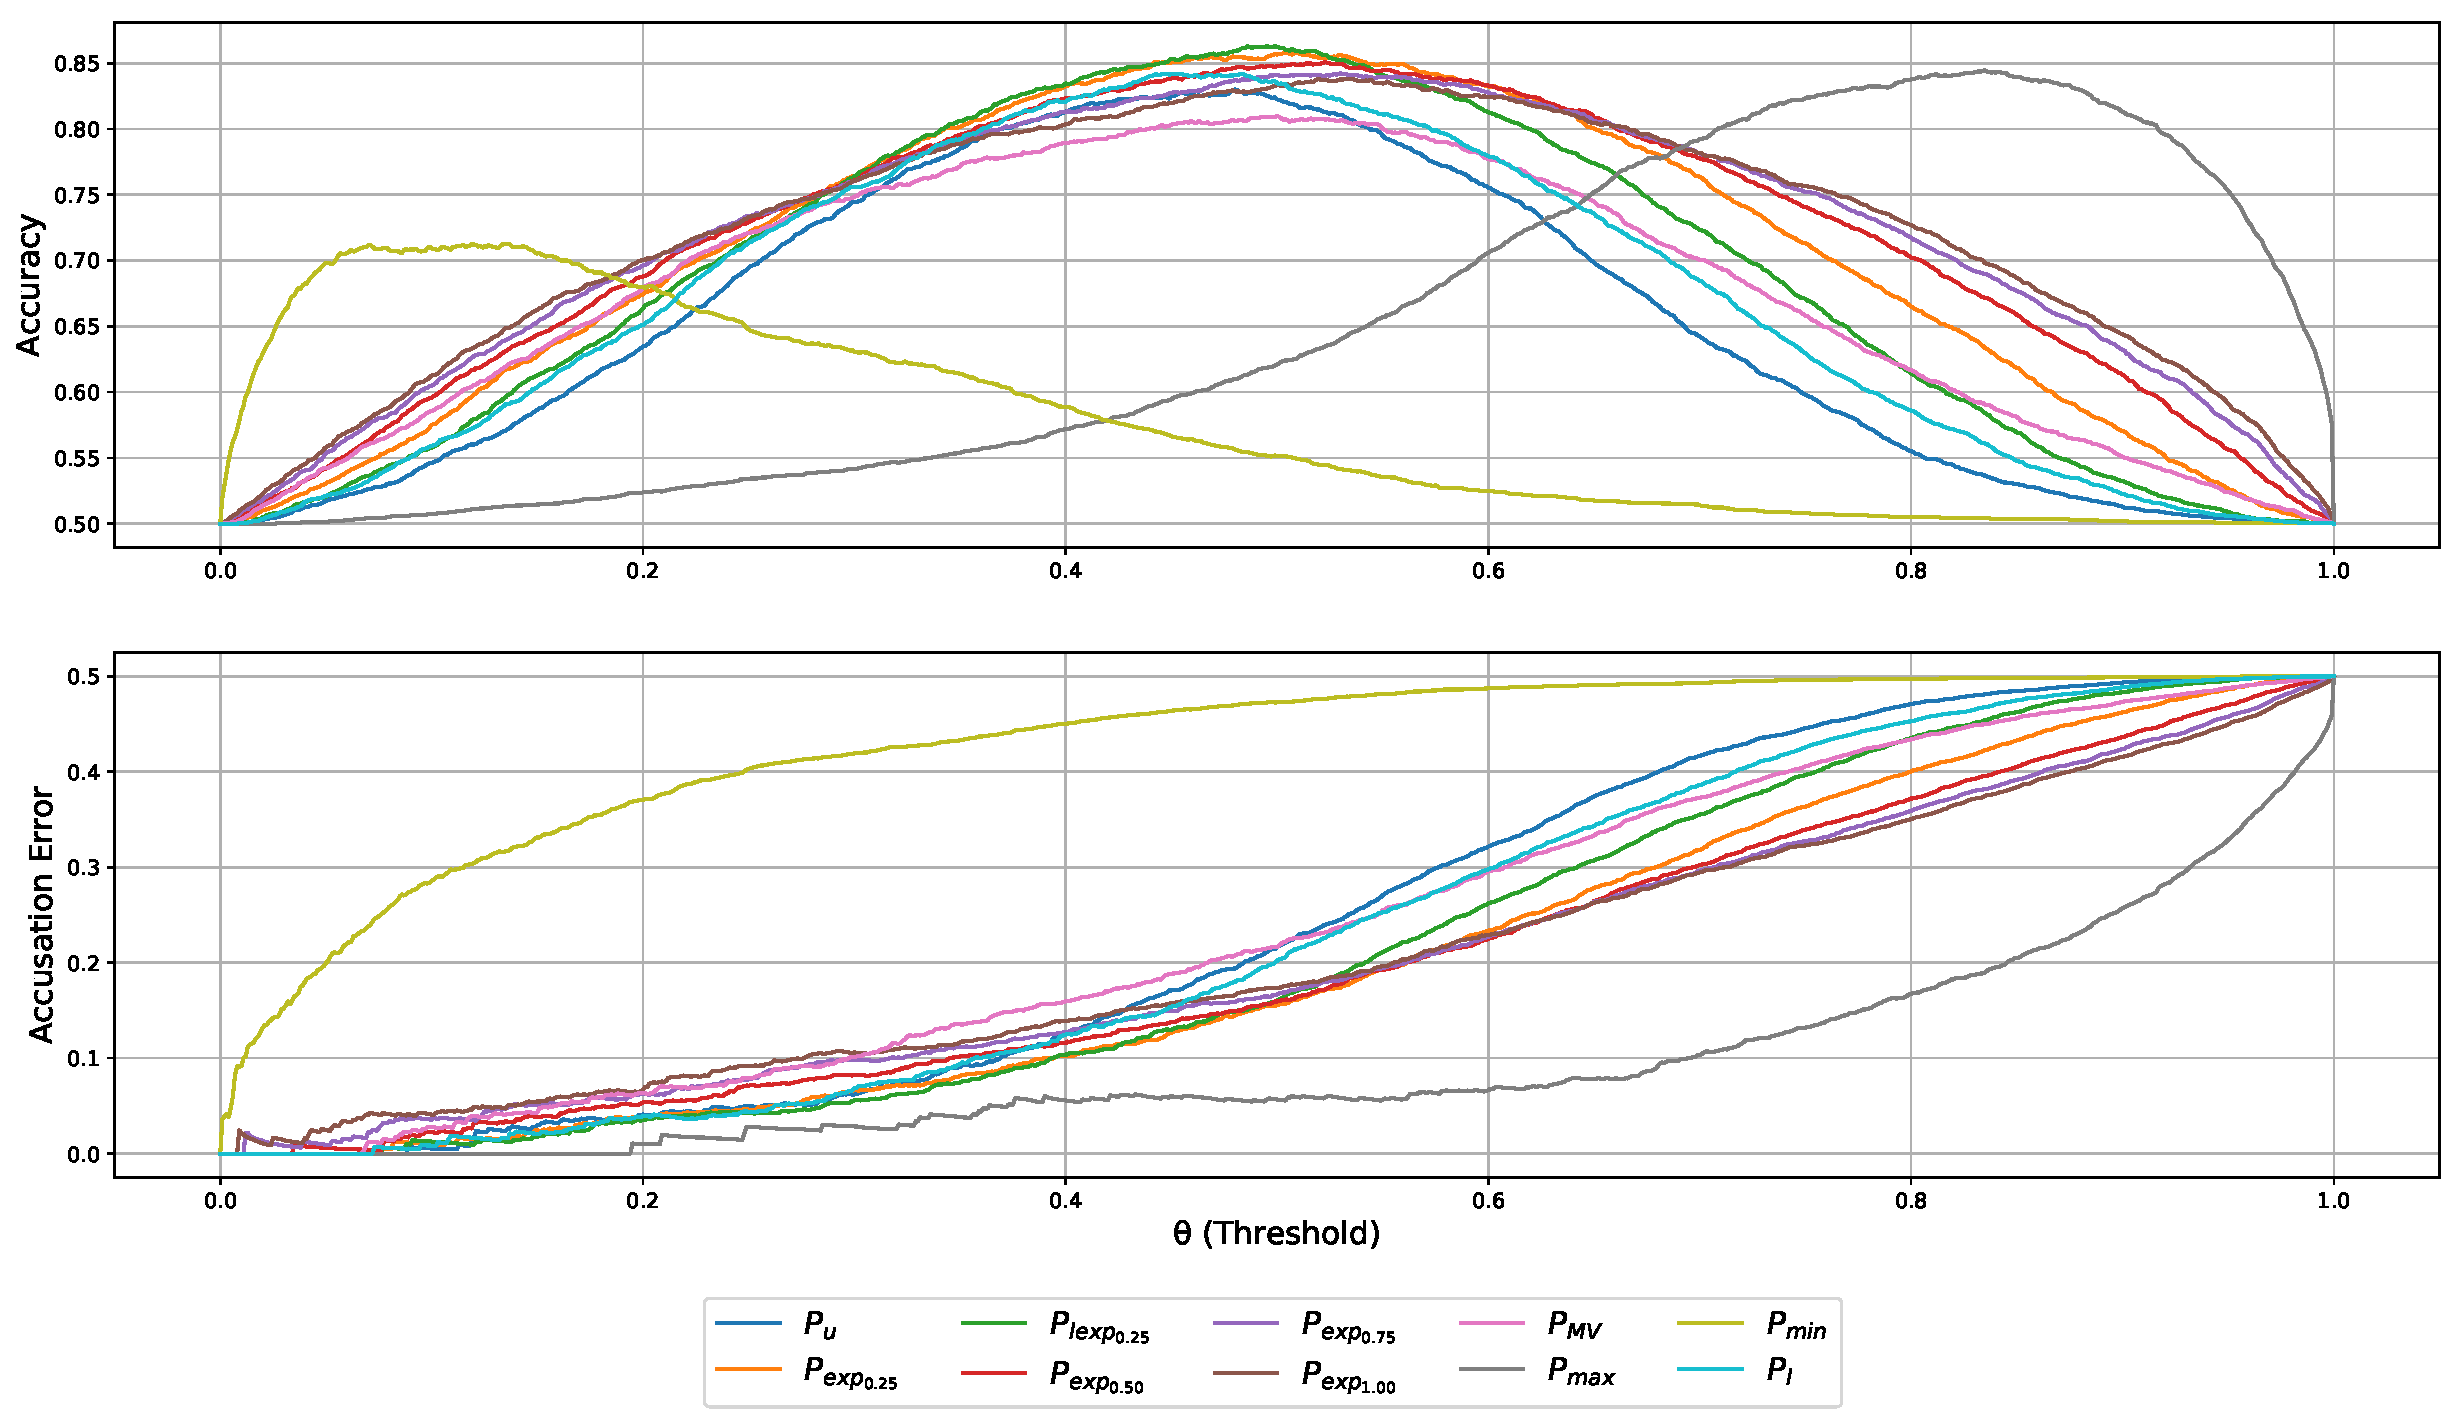
\includegraphics[scale=0.33]{./pictures/experiments/conv_char_nn/prediction_system_50}
    \caption{Results of running the prediction system with the network described
        in Section \ref{subsubsec:conv_char_nn} on a validation dataset with
        50\% positive samples and 50\% negative samples. In the upper graph we
        show the accuracies obtained as a function of $\theta$ for different
        weights $w$. At the bottom we have shown the accusation error as a
        function $\theta$ again with one line for each weight. We can see that
        as the threshold increases and we accuse more people of cheating the
        accusation error rises.}
    \label{fig:conv-char-NN-pred-50}
\end{figure}

\begin{figure}
    \centering
    \textbf{Prediction System Results for 0.04 Split, \glsdesc{conv-char-NN}}\par\medskip
    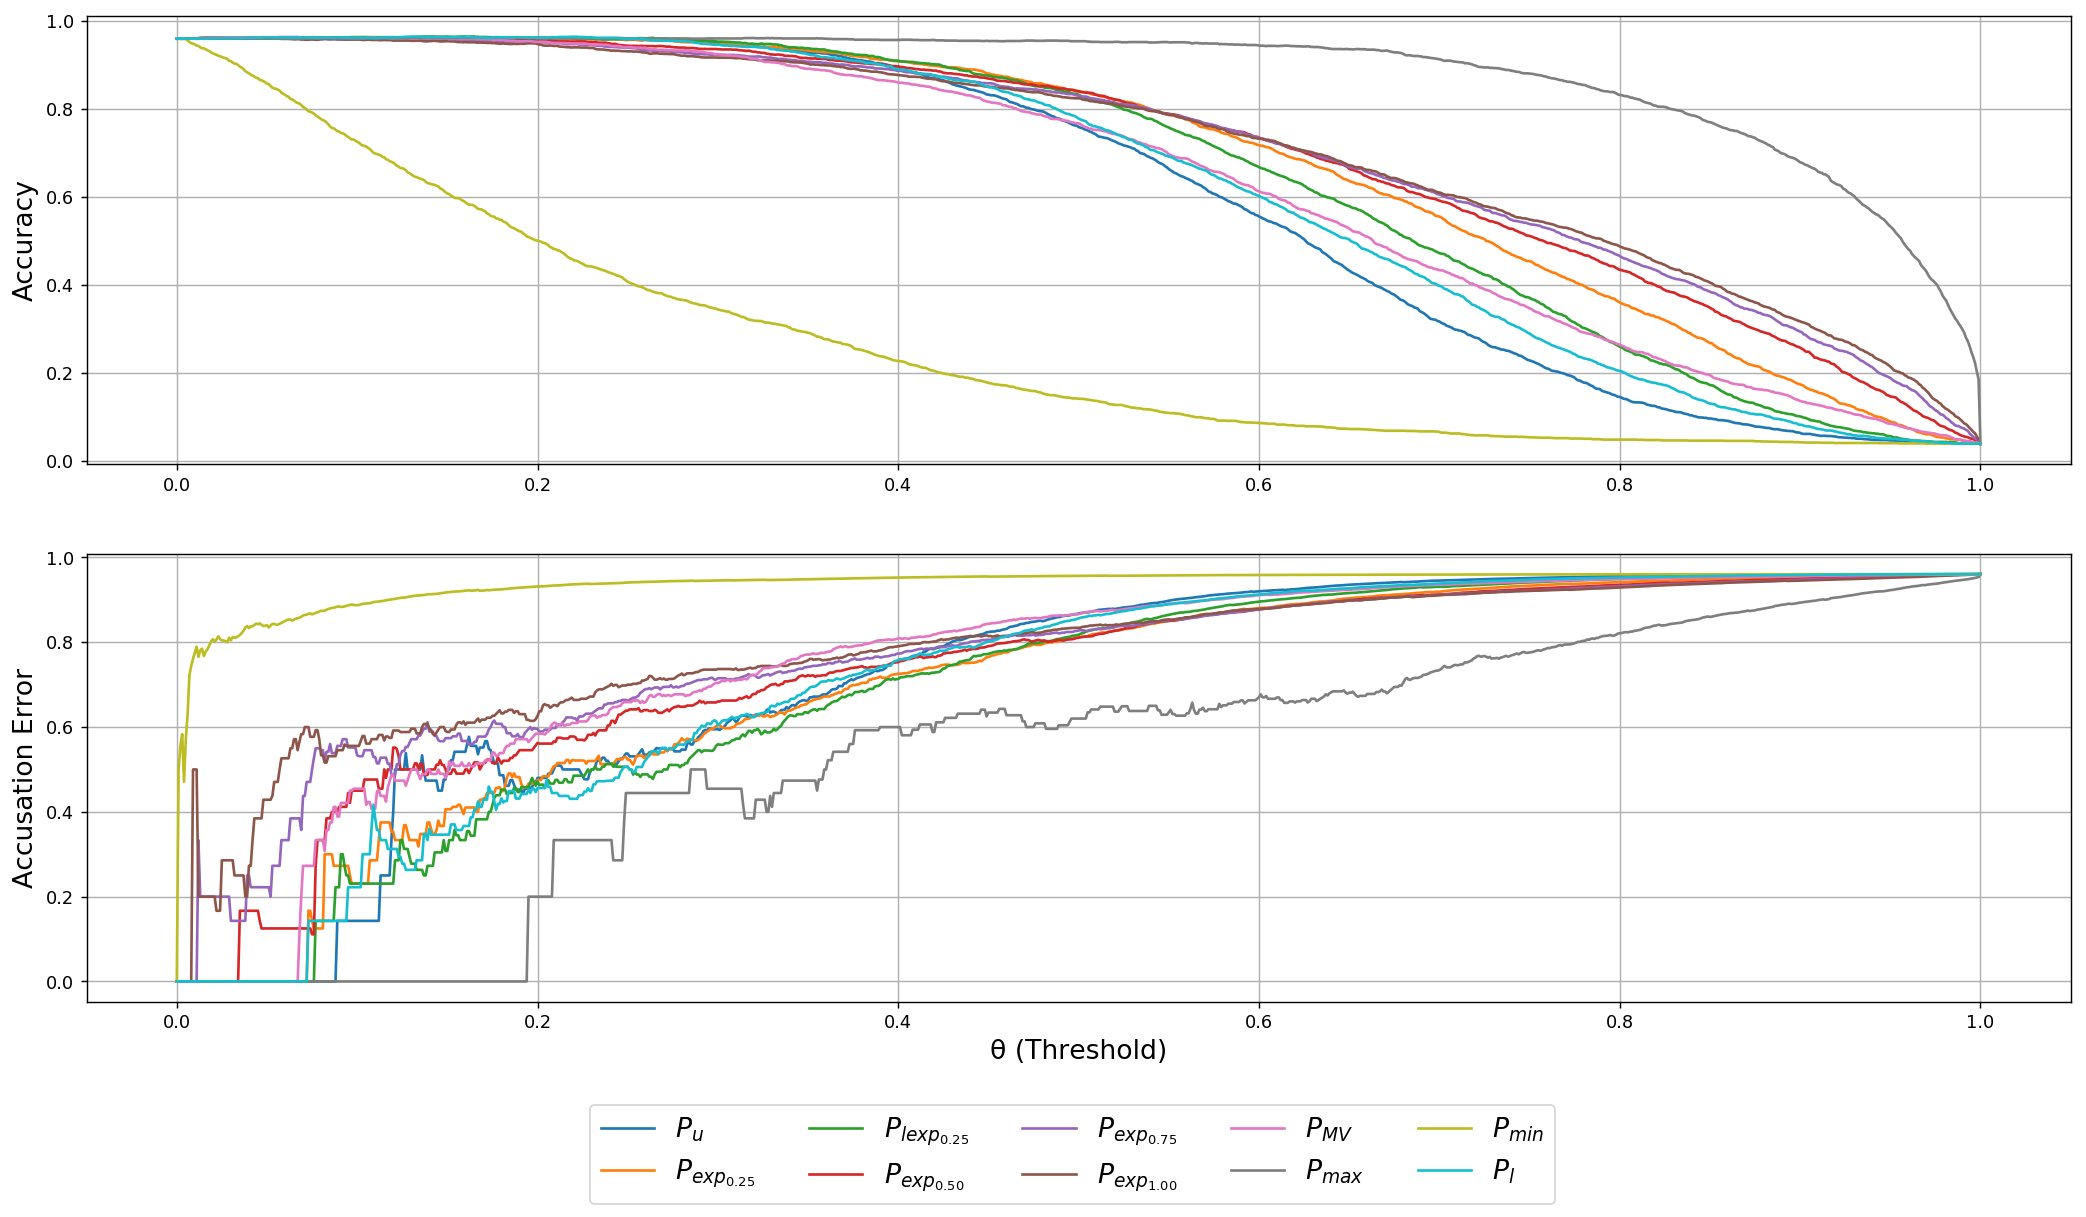
\includegraphics[scale=0.33]{./pictures/experiments/conv_char_nn/prediction_system_04}
    \caption{Results of running the prediction system with the network described
        in Section \ref{subsubsec:conv_char_nn} on a validation dataset with
        96\% positive samples and 4\% negative samples. In the upper graph we
        show the accuracies obtained as a function of $\theta$ for different
        weights $w$. At the bottom we have shown the accusation error as a
        function $\theta$ again with one line for each weight. We can see that
        as the threshold increases and we accuse more people of cheating the
        accusation error rises.}
    \label{fig:conv-char-NN-pred-4}
\end{figure}

The best configuration for both the 50/50 split and 96/04 split was the
following,

\begin{center}
\begin{tabular}{|c|c|c|c|c|c|c|c|c|}
\hline
Split & Weight            & $\theta$ & TP  & TN  & FP & FN & Acc    & A-Error \\ \hline
50/50 & $P_{lexp_{0.25}}$ & 0.390    & 1843 & 1482 & 517 & 156 & 0.8316 & 0.095   \\ \hline
96/04 & $P_{mv}$          & 0.057    & 1999 & 8    & 74  & 0   & 0.9644 & 0.000   \\ \hline
\end{tabular}
\end{center}

\subsubsection{\glsdesc{rec-sent-NN}}
\label{subsubsec:prediction_system_rec-sent-NN}

The second network we tuned hyperparameters for was the network depicted in
\ref{fig:rec-sent-NN}. This network was the one \gls{RNN} we attempted to use
to solve this problem. Applying the prediction system to this network gave the
results which can be seen in the Figures, \ref{fig:rec-sent-NN-pred-50} and
\ref{fig:rec-sent-NN-pred-4}

\begin{figure}
    \centering
    \textbf{Prediction System Results for 0.5 Split, \glsdesc{rec-sent-NN}}\par\medskip
    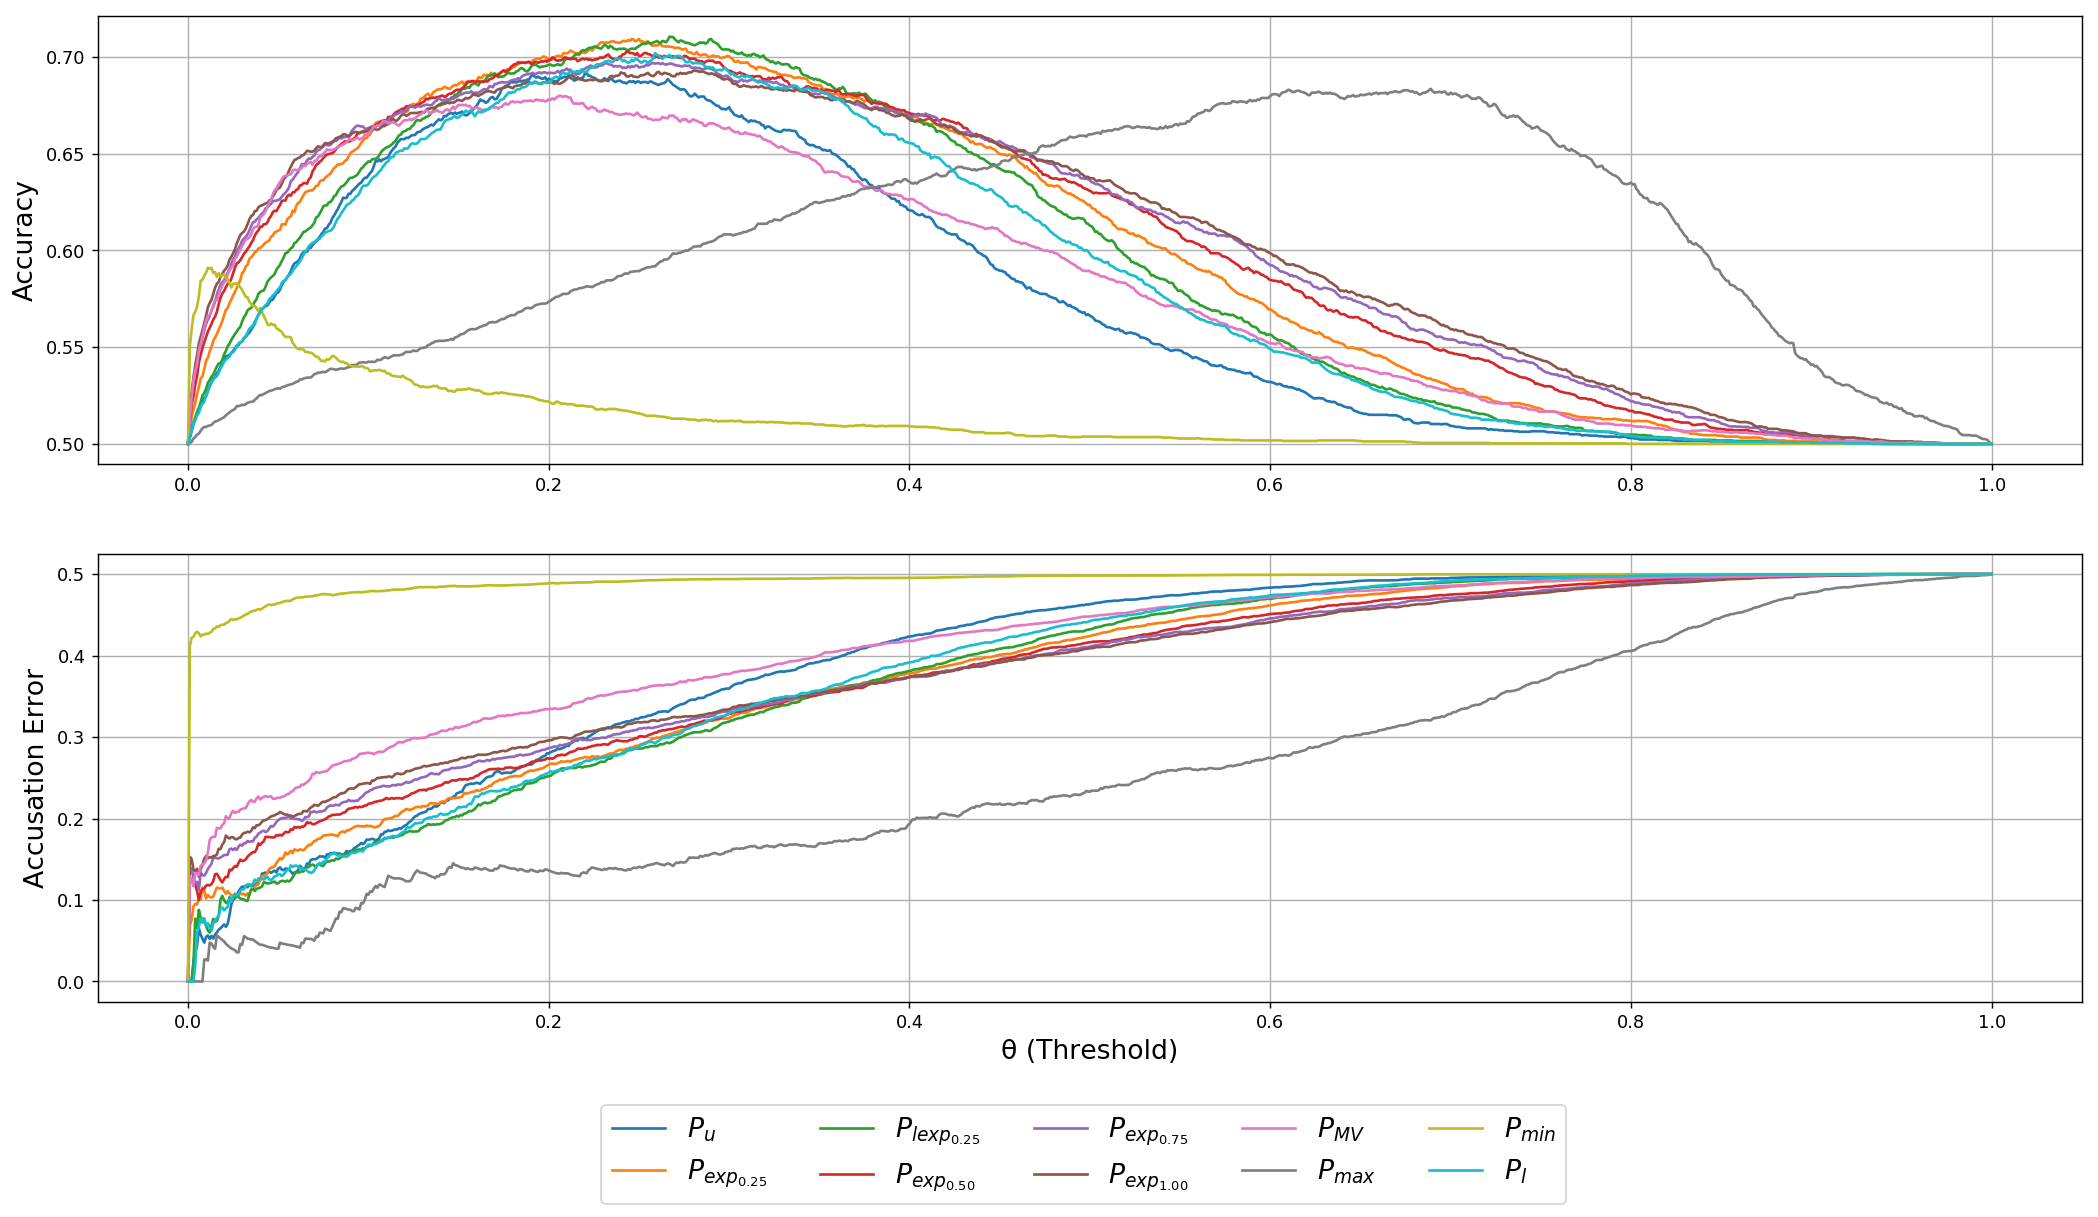
\includegraphics[scale=0.33]{./pictures/experiments/rec_sent_nn/prediction_system_50}
    \caption{Results of running the prediction system with the network described
        in Section \ref{subsubsec:rec_sent_nn} on a validation dataset
        with 50\% positive samples and 50\% negative samples. In the upper graph
        we show the accuracies obtained as a function of $\theta$ for different
        weights $w$. At the bottom we have shown the accusation error as a
        function $\theta$ again with one line for each weight. We can see that
        as the threshold increases and we accuse more people of cheating the
        accusation error rises.}
    \label{fig:rec-sent-NN-pred-50}
\end{figure}

\begin{figure}
    \centering
    \textbf{Prediction System Results for 0.04 Split, \glsdesc{rec-sent-NN}}\par\medskip
    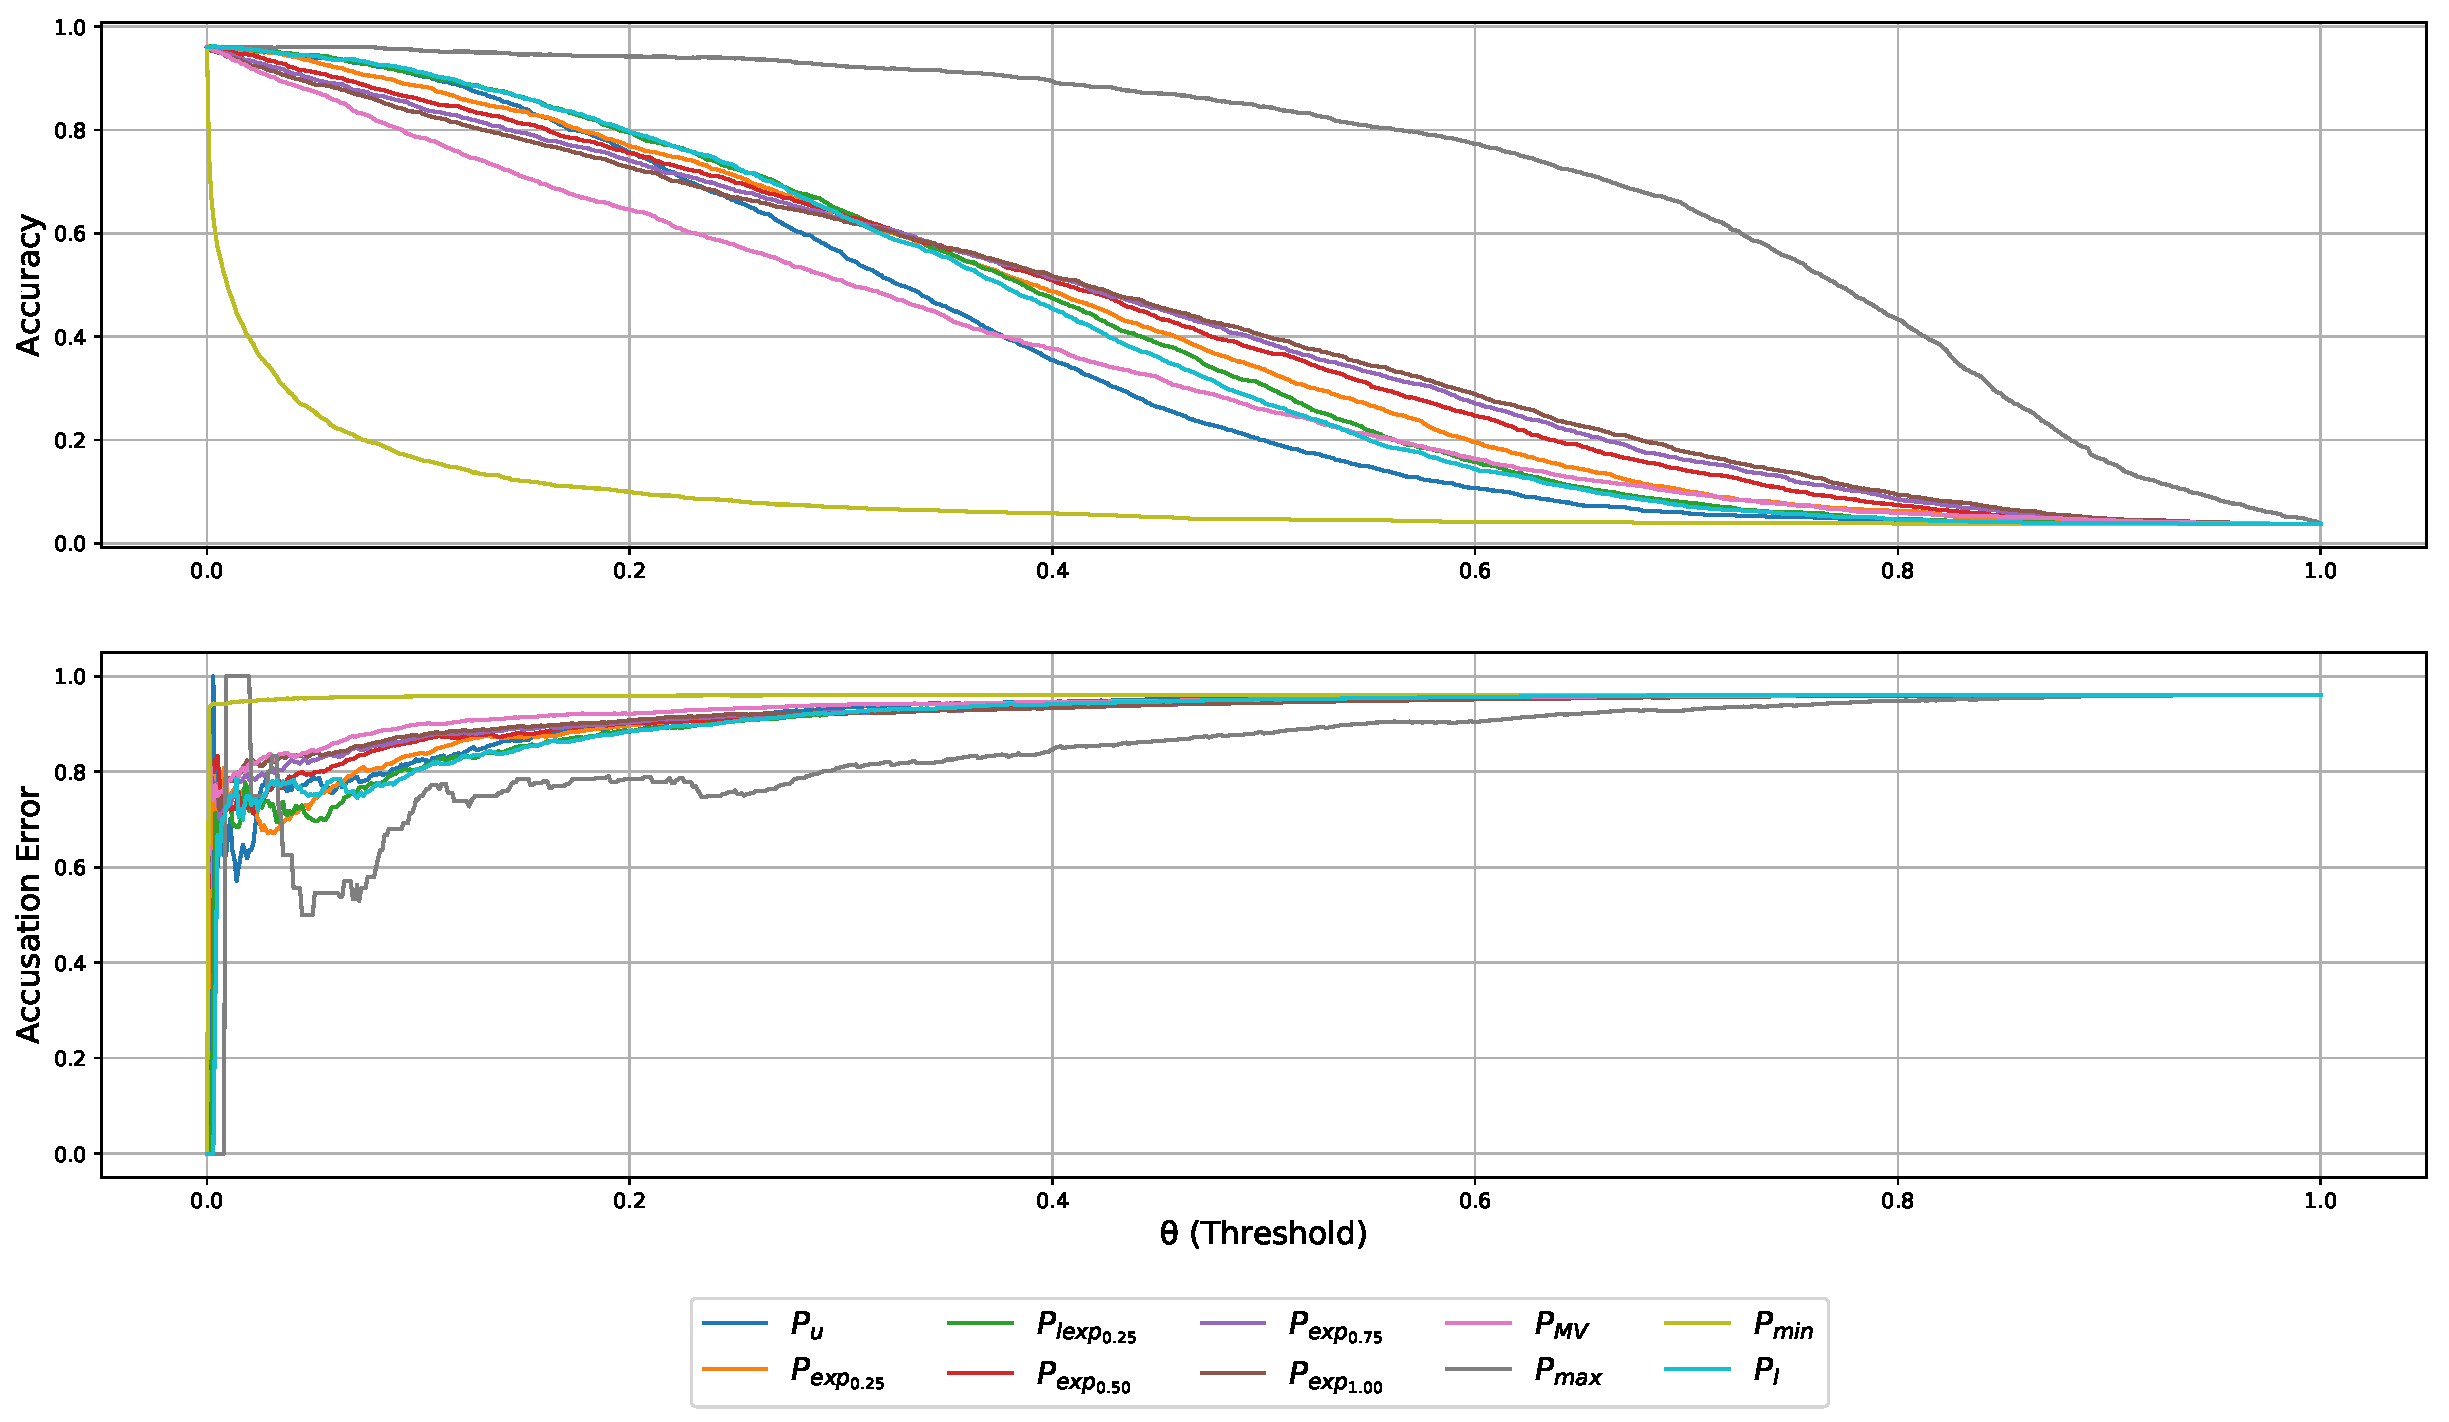
\includegraphics[scale=0.33]{./pictures/experiments/rec_sent_nn/prediction_system_04}
    \caption{Results of running the prediction system with the network described
        in Section \ref{subsubsec:rec_sent_nn} on a validation dataset
        with 96\% positive samples and 4\% negative samples. In the upper graph
        we show the accuracies obtained as a function of $\theta$ for different
        weights $w$. At the bottom we have shown the accusation error as a
        function $\theta$ again with one line for each weight. We can see that
        as the threshold increases and we accuse more people of cheating the
        accusation error rises.}
    \label{fig:rec-sent-NN-pred-4}
\end{figure}

The best configurations for \gls{rec-sent-NN}, using both the 50/50 and
96/04 split of data was the following,
\begin{center}
\begin{tabular}{|c|c|c|c|c|c|c|c|c|}
\hline
Split & Weight            & $\theta$ & TP  & TN & FP  & FN & Acc    & A-Error \\ \hline
50/50 & $P_{lexp_{0.25}}$ & 0.033    & 1965 & 310 & 1689 & 34  & 0.5690 & 0.099   \\ \hline
96/04 & $P_{lexp_{0.25}}$ & 0.002    & 1999 & 1   & 79   & 0   & 0.9620 & 0.000   \\ \hline
\end{tabular}
\end{center}

These result are to expected when looking at the graphs. The immediate spike in
accusation error leaves the model very little room to increase the accuracy in.
This is most likely the result of the aforementioned author specific learning
the network does.


\subsubsection{\glsdesc{conv-char-word-NN}}
\label{subsubsec:prediction_system_conv-char-word-NN}

The third network we tuned hyperparameters for was the network presented
in Figure TODO. The network used convolutions on the character level and
word level to extract features and used a dense network to decide whether or
not the texts were written by the same author. We have shown the accuracy
and accusation error for the dataset containing 50\% negatives in Figure
\ref{fig:conv-char-word-NN-pred-50} and for the dataset containing 4\%
negatives in Figure \ref{fig:conv-char-word-NN-pred-4}.

\begin{figure}
    \centering
    \textbf{Prediction System Results for 0.5 Split, \glsdesc{conv-char-word-NN}}\par\medskip
    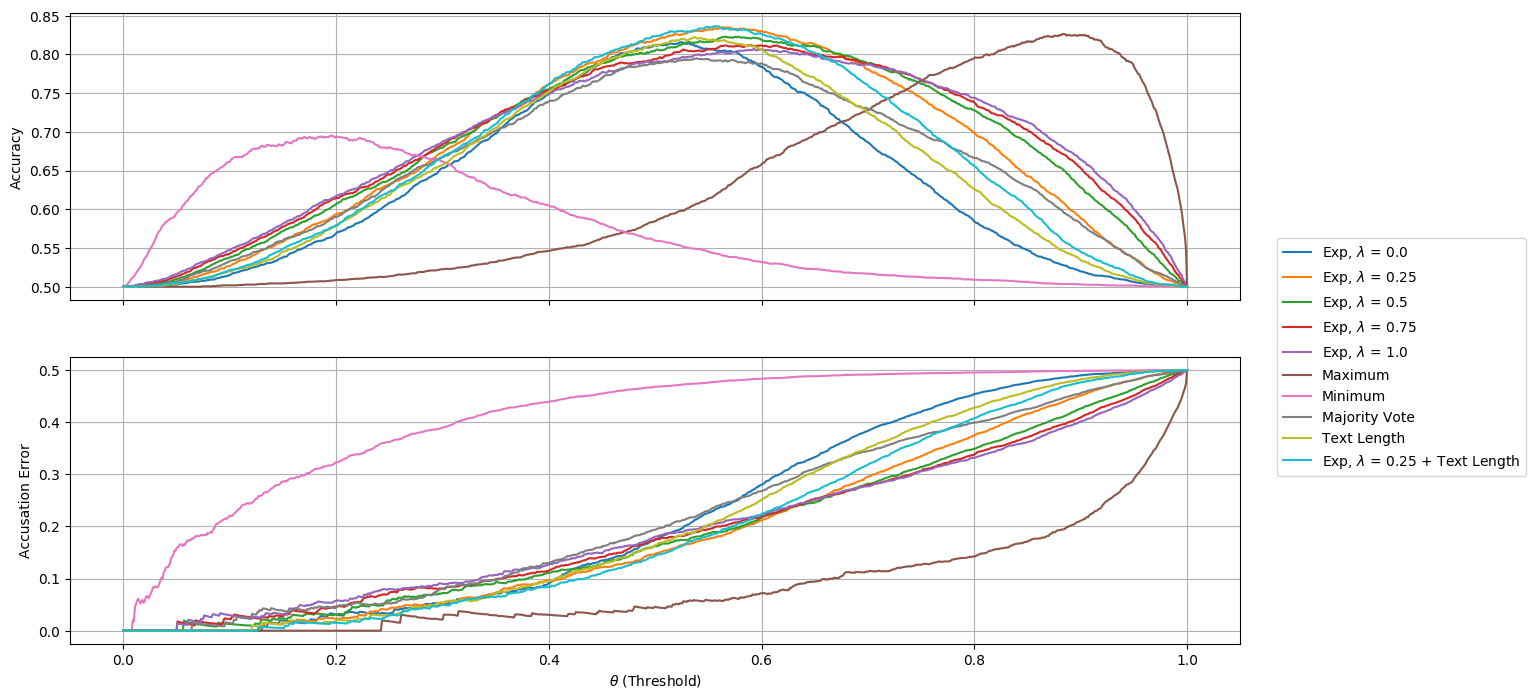
\includegraphics[scale=0.33]{./pictures/experiments/conv_char_word_nn/prediction_system_50}
    \caption{Results of running the prediction system with the network described
        in Section \ref{subsubsec:conv_char_word_nn} on a validation dataset
        with 50\% positive samples and 50\% negative samples. In the upper graph
        we show the accuracies obtained as a function of $\theta$ for different
        weights $w$. At the bottom we have shown the accusation error as a
        function $\theta$ again with one line for each weight. We can see that
        as the threshold increases and we accuse more people of cheating the
        accusation error rises.}
    \label{fig:conv-char-word-NN-pred-50}
\end{figure}

\begin{figure}
    \centering
    \textbf{Prediction System Results for 0.04 Split, \glsdesc{conv-char-word-NN}}\par\medskip
    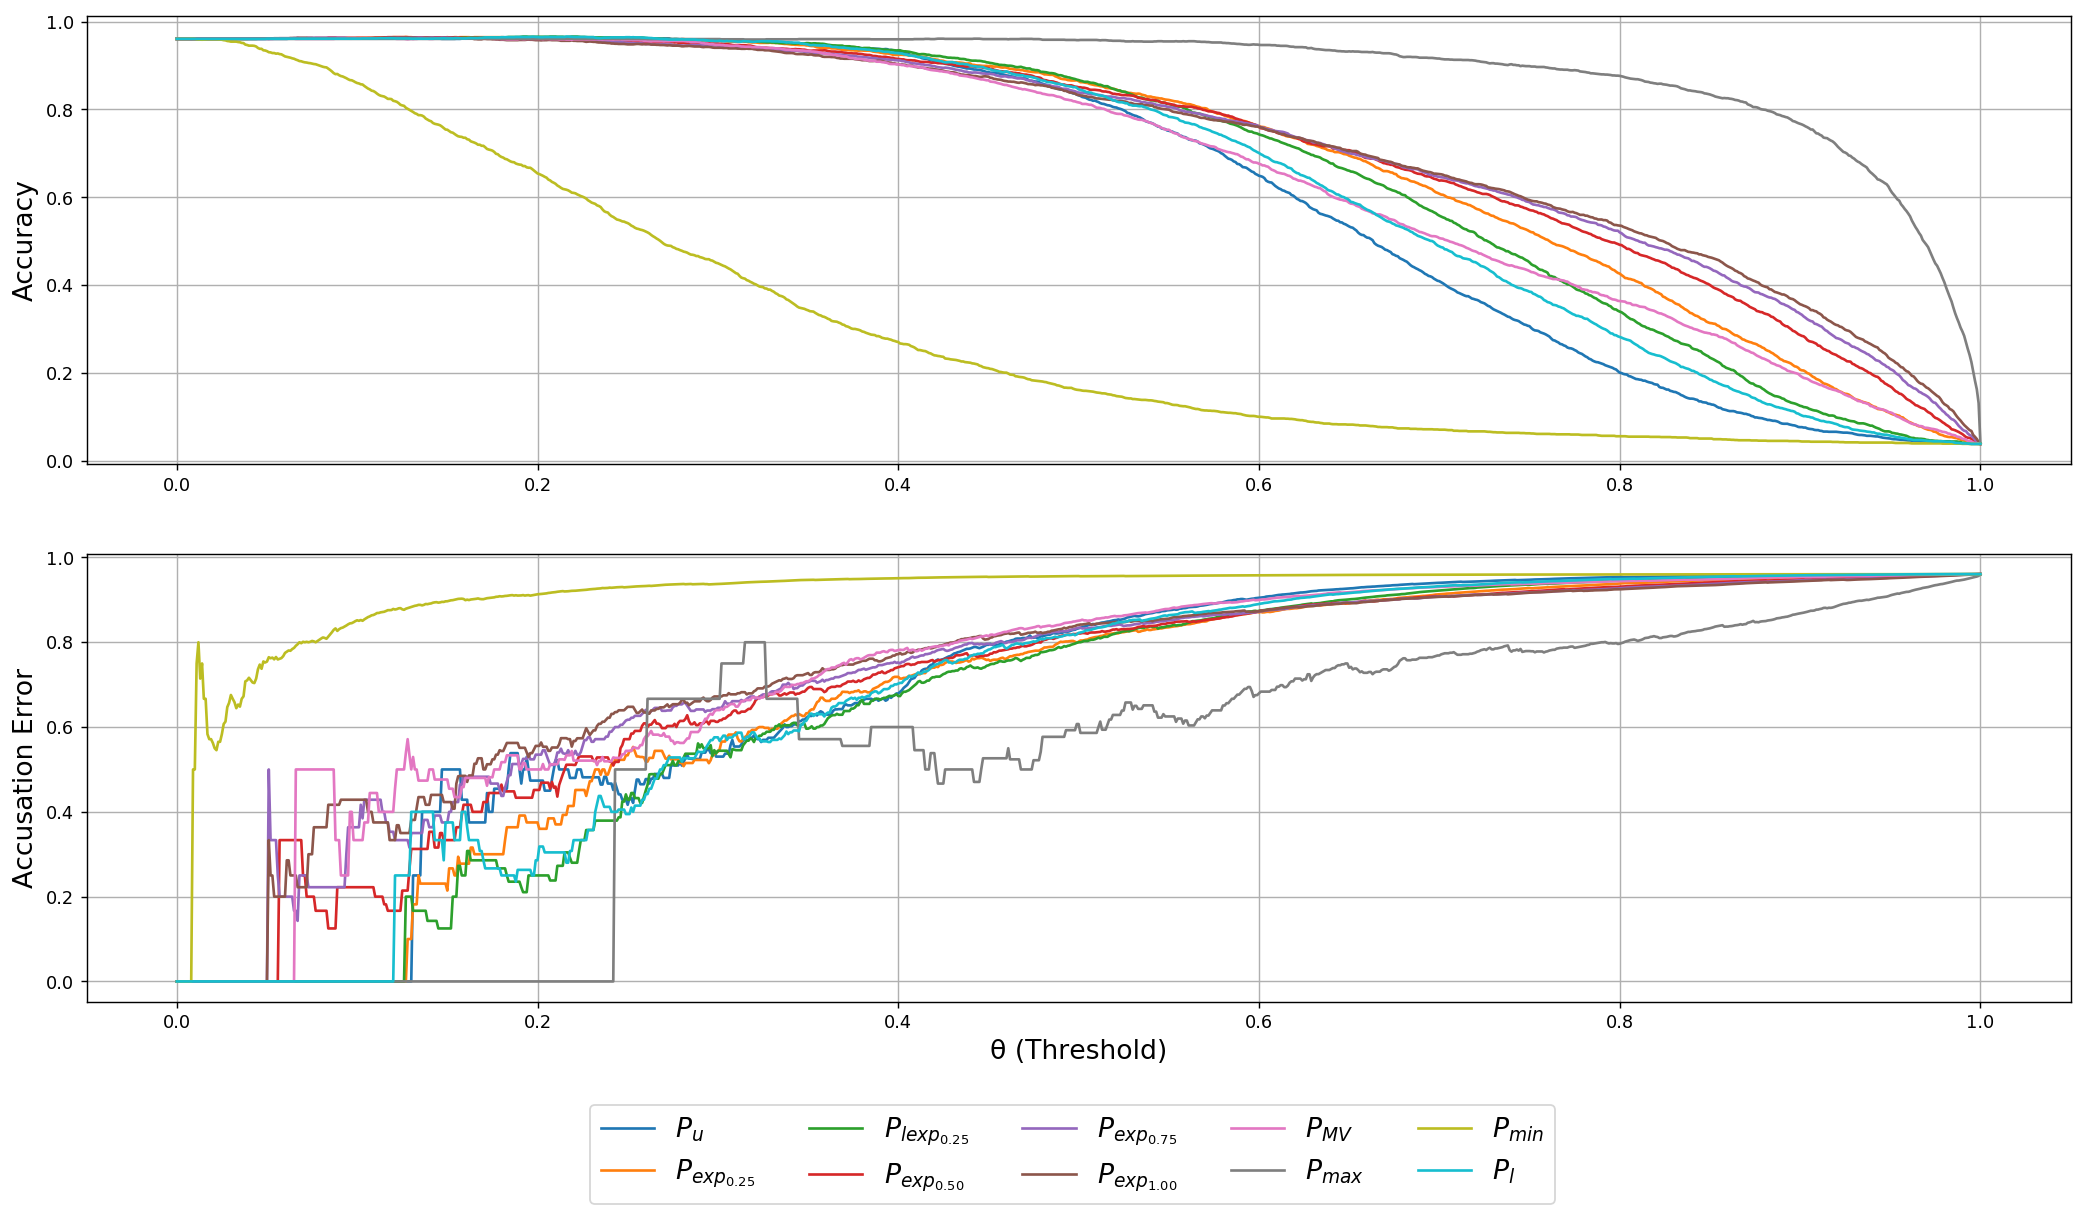
\includegraphics[scale=0.33]{./pictures/experiments/conv_char_word_nn/prediction_system_04}
    \caption{Results of running the prediction system with the network described
        in Section \ref{subsubsec:conv_char_word_nn} on a validation dataset
        with 96\% positive samples and 4\% negative samples. In the upper graph
        we show the accuracies obtained as a function of $\theta$ for different
        weights $w$. At the bottom we have shown the accusation error as a
        function $\theta$ again with one line for each weight. We can see that
        as the threshold increases and we accuse more people of cheating the
        accusation error rises.}
    \label{fig:conv-char-word-NN-pred-4}
\end{figure}

The best configuration for the 50/50 split and the 96/04 split was the
following,

\begin{center}
\begin{tabular}{|c|c|c|c|c|c|c|c|c|}
\hline
Split & Weight            & $\theta$ & TP  & TN  & FP & FN & Acc     & A-Error \\ \hline
50/50 & $P_{lexp_{0.25}}$ & 0.433    & 1856 & 1302 & 697 & 143 & 0.7898 & 0.099   \\ \hline
96/04 & $P_{exp_{0.25}}$  & 0.127    & 1999 & 9    & 73  & 0   & 0.9649 & 0.000   \\ \hline
\end{tabular}
\end{center}

A summarizing view of the validation performance of the different networks can
be seen in Table \ref{tab:experi-results}.

\begin{table}[h]
\begin{tabular}{|c|c|c|c|c|c|c|c|c|c|}
\hline
Split                  & Network                 & Weight            & $\theta$ & TP  & TN  & FP  & FN & Acc     & A-Error \\ \hline
\multirow{3}{*}{50/50} & \gls{conv-char-NN}      & $P_{lexp_{0.25}}$ & 0.390    & 1843 & 1482 & 517  & 156 & 0.8316 & 0.095   \\ \cline{2-10} 
                       & \gls{rec-sent-NN}       & $P_{lexp_{0.25}}$ & 0.033    & 1965 & 310  & 1689 & 34  & 0.5690 & 0.099   \\ \cline{2-10} 
                       & \gls{conv-char-word-NN} & $P_{lexp_{0.25}}$ & 0.433    & 1856 & 1302 & 697  & 143 & 0.7898 & 0.099   \\ \hline
\multirow{3}{*}{96/04} & \gls{conv-char-NN}      & $P_{mv}$          & 0.057    & 1999 & 8    & 74   & 0   & 0.9644 & 0.000   \\ \cline{2-10} 
                       & \gls{rec-sent-NN}       & $P_{lexp_{0.25}}$ & 0.002    & 1999 & 1    & 79   & 0   & 0.9620 & 0.000   \\ \cline{2-10} 
                       & \gls{conv-char-word-NN} & $P_{exp_{0.25}}$  & 0.127    & 1999 & 9    & 73   & 0   & 0.9649 & 0.000   \\ \hline
\end{tabular}
\caption{A summarizing view of the performance of the different networks on the
the validation dataset (F).}
\label{tab:experi-results}
\end{table}
